% toolsoftrade/toolsoftrade.tex
% mainfile: ../perfbook.tex
% SPDX-License-Identifier: CC-BY-SA-3.0

\QuickQuizChapter{chp:Tools of the Trade}{Tools of the Trade}{qqztoolsoftrade}
%
\Epigraph{You are only as good as your tools, and your tools are only
	  as good as you are.}{\emph{Unknown}}

이 챕터는 병렬 프로그래밍 트레이드오프에 사용되는 일부 기본적 도구들을 주로
리눅스와 비슷한 운영체제에서 수행되는 어플리케이션에서 사용할 수 있는 것들에
초점을 맞춰 소개합니다.
Section~\ref{sec:toolsoftrade:Scripting Languages} 에서 스크립트 언어로
시작해서,
Section~\ref{sec:toolsoftrade:POSIX Multiprocessing} 에서는 POSIX API 에 의해
지원되는 멀티 프로세스 병렬성을 설명하고 POSIX 쓰레드를 다룬 후,
Section~\ref{sec:toolsoftrade:Alternatives to POSIX Operations}
에서는 다른 환경에서의 비슷한 것들을 다룬 후, 마지막으로
Section~\ref{sec:toolsoftrade:The Right Tool for the Job: How to Choose?}
에서는 일을 해결해 줄 도구를 고르는 걸 돕습니다.

\iffalse

This chapter provides a brief introduction to some basic tools of the
parallel-programming trade, focusing mainly on those available to
user applications running on operating systems similar to Linux.
Section~\ref{sec:toolsoftrade:Scripting Languages} begins with
scripting languages,
Section~\ref{sec:toolsoftrade:POSIX Multiprocessing}
describes the multi-process parallelism supported by the POSIX API and
touches on POSIX threads,
Section~\ref{sec:toolsoftrade:Alternatives to POSIX Operations}
presents analogous operations in other environments, and finally,
Section~\ref{sec:toolsoftrade:The Right Tool for the Job: How to Choose?}
helps to choose the tool that will get the job done.

\fi

\QuickQuiz{
	이것들을 도구라고 부르시나요???
	이것들은 제게는 그보다는 저수준 (low-level) 동기화 도구들처럼
	보이는데요!

	\iffalse

	You call these tools???
	They look more like low-level synchronization primitives to me!

	\fi

}\QuickQuizAnswer{
	그것들은 실제로 저수준 동기화 도구들이기 때문에 그렇게 보일 겁니다.
	그리고 그것들은 실제로 저수준 동시성 소프트웨어를 만들기 위한 기본적
	도구들입니다.

	\iffalse

	They look that way because they are in fact low-level synchronization
	primitives.
	And they are in fact the fundamental tools for building low-level
	concurrent software.

	\fi

}\QuickQuizEnd

이 챕터는 간단한 소개를 제공할 뿐임을 알아두시기 바랍니다.
더 자세한 것들은 참조문헌에서 (그리고 인터넷에서) 얻을 수 있으며, 더 많은
정보들이 뒤의 챕터들에서 제공될 겁니다.

\iffalse

Please note that this chapter provides but a brief introduction.
More detail is available from the references (and from the Internet),
and more information will be provided in later chapters.

\fi

\section{Scripting Languages}
\label{sec:toolsoftrade:Scripting Languages}
%
\epigraph{The supreme excellence is simplicity.}
	 {\emph{Henry Wadsworth Longfellow, simplified}}
% The original:
% "In character, in manner, in style, in all things, the supreme
% excellence is simplicity."

리눅스 셸 스크립트는 병렬성을 다루는 간단하지만 효과적인 방법들을 제공합니다.
예를 들어, 여러분이 \co{compute_it} 이라는 프로그램이 있고 이걸 두개의 다른
인자 집합을 가지고 두번 수행시켜야 한다고 생각해 봅시다.
이걸 UNIX 셸 스크립트를 이용해서 다음과 같이 해낼 수 있습니다:

\iffalse

The Linux shell scripting languages provide simple but effective ways
of managing parallelism.
For example, suppose that you had a program \co{compute_it}
that you needed to run twice with two different sets of arguments.
This can be accomplished using UNIX shell scripting as follows:

\fi

\input{CodeSamples/toolsoftrade/parallel@compute_it.fcv}

\begin{figure}[tb]
\centering
\resizebox{3in}{!}{\includegraphics{toolsoftrade/shellparallel}}
\caption{Execution Diagram for Parallel Shell Execution}
\label{fig:toolsoftrade:Execution Diagram for Parallel Shell Execution}
\end{figure}

\begin{fcvref}[ln:toolsoftrade:parallel:compute_it]
라인~\lnref{comp1} 과~\lnref{comp2} 는 이 프로그램을 두번 실행시키고, 이것들의
결과물을 두개의 별도의 파일에 저장하는데 \co{&} 문자는 셸에게 이 두 프로그램
실행을 백그라운드에서 하도록 지시합니다.
라인~\lnref{wait} 은 이 두개의 실행이 완료되기를 기다리고, 라인~\lnref{cat1}
과~\lnref{cat2} 는 그 결과를 출력합니다.
\end{fcvref}
그렇게 진행되는 실행과정이
Figure~\ref{fig:toolsoftrade:Execution Diagram for Parallel Shell Execution}
에 보여져 있습니다:
\co{compute_it} 의 두 실행은 병렬로 진행되며, \co{wait} 은 이 두 실행이 모두
끝난 후 종료되며, 이후에는 두번의 \co{cat} 실행이 순차적으로 이루어집니다.

\iffalse

\begin{fcvref}[ln:toolsoftrade:parallel:compute_it]
Lines~\lnref{comp1} and~\lnref{comp2} launch two instances of this
program, redirecting their
output to two separate files, with the \co{&} character directing the
shell to run the two instances of the program in the background.
Line~\lnref{wait} waits for both instances to complete, and
lines~\lnref{cat1} and~\lnref{cat2}
display their output.
\end{fcvref}
The resulting execution is as shown in
Figure~\ref{fig:toolsoftrade:Execution Diagram for Parallel Shell Execution}:
the two instances of \co{compute_it} execute in parallel,
\co{wait} completes after both of them do, and then the two instances
of \co{cat} execute sequentially.
% @@@ Maui scheduler, load balancing, BOINC, and so on.
% @@@ Diagram showing parallel execution.

\fi

\QuickQuizSeries{%
\QuickQuizB{

	하지만 이 웃긴 셸 스크립트는 \emph{진짜} 병렬 프로그램이 아니예요!
	왜 이런 사소한 걸 신경쓰죠???

	\iffalse

	But this silly shell script isn't a \emph{real} parallel program!
	Why bother with such trivia???

	\fi

}\QuickQuizAnswerB{
	여러분은 \emph{절대} 간단한 것을 잊지 말아야 하기 때문입니다!

	이 책의 제목은
	``Is Parallel Programming Hard, And, If So, What Can You Do About It?''
	임을 명심하시기 바랍니다.
	이를 위해 여러분이 할 수 있는 가장 효과적인 일은 간단한 걸 잊는 걸
	예방하는 겁니다!
	어쨌건, 여러분이 병렬 프로그래밍을 어려운 방식으로 할 것을 선택한다면,
	여러분 스스로밖에는 욕할 사람이 없을 겁니다.

	\iffalse

	Because you should \emph{never} forget the simple stuff!

	Please keep in mind that the title of this book is
	``Is Parallel Programming Hard, And, If So, What Can You Do About It?''.
	One of the most effective things you can do about it is to
	avoid forgetting the simple stuff!
	After all, if you choose to do parallel programming the hard
	way, you have no one but yourself to blame.

	\fi

}\QuickQuizEndB
%
\QuickQuizE{
	병렬 셸 스크립트를 작성할 수 있는 더 간단한 방법이 있을까요?
	있다면, 어떻게 하죠?  없다면, 왜 없죠?

	\iffalse

	Is there a simpler way to create a parallel shell script?
	If so, how?  If not, why not?

	\fi
}\QuickQuizAnswerE{
	간단한 한가지 방법은 셸 파이프라인을 사용하는 겁니다:

	\iffalse

	One straightforward approach is the shell pipeline:

	\fi

\begin{VerbatimU}
grep $pattern1 | sed -e 's/a/b/' | sort
\end{VerbatimU}

	충분히 큰 입력 파일에 대해서, \co{grep} 은 패턴 매칭을 \co{sed} 가
	수정을 하고 \co{sort} 가 입력을 처리하는 동안 병렬로 수행할 겁니다.
	셸 스크립트의 병렬성과 파이프라인 방식에 대한 데모를 위해
	\path{parallel.sh} 파일을 보시기 바랍니다.

	\iffalse

	For a sufficiently large input file,
	\co{grep} will pattern-match in parallel with \co{sed}
	editing and with the input processing of \co{sort}.
	See the file \path{parallel.sh} for a demonstration of
	shell-script parallelism and pipelining.

	\fi

}\QuickQuizEndE
}

또다른 예로, 소프트웨어 빌드 스크립트 언어인 \co{make} 는 이 빌드 과정에
얼만큼의 병렬성이 사용되어야 할지 명세하는 \co{-j} 옵션을 제공합니다.
따라서, 리눅스 커널을 빌드할 때 \co{make -j4} 를 타이핑 하는 것은 최대 네개의
빌드 과정이 동시에 수행되도록 합니다.

이 간단한 예제들을 통해 병렬 프로그래밍은 항상 복잡하거나 어려워야 할 필요는
없다는 것을 여러분이 받아들이길 바랍니다.

\iffalse

For another example, the \co{make} software-build scripting language
provides a \co{-j} option that specifies how much parallelism should be
introduced into the build process.
Thus, typing \co{make -j4} when building a Linux kernel specifies that
up to four build steps be executed concurrently.

It is hoped that these simple examples convince you that parallel
programming need not always be complex or difficult.

\fi

\QuickQuiz{
	하지만 스크립트 기반의 병렬 프로그래밍이 그렇게 쉽다면, 다른 것들에
	신경쓰는 이유가 뭔가요?

	\iffalse

	But if script-based parallel programming is so easy, why
	bother with anything else?

	\fi

}\QuickQuizAnswer{
	사실, 오늘날 사용되는 병렬 프로그램들 중 많은 것들이 스크립트 기반일
	가능성이 무척 높습니다.
	하지만, 스크립트 기반 병렬성은 나름의 한계를 가지고 있습니다:
	\begin{enumerate}
	\item	새로운 프로세스의 생성은 \co{fork()} 와 \co{exec()} 이라는 비싼
		시스템 콜을 사용하기 때문에 무척 무거운 작업입니다.
	\item	데이터 공유와 파이프라이닝의 포함은 보통 비싼 파일 I/O 를
		사용되게 합니다.
	\item	스크립트에서 사용할 수 있는 안정적인 동기화 도구들은 일반적으로
		비싼 파일 I/O 를 사용되게 합니다.
	\item	스크립트 언어는 너무 느린 경우가 많습니다, 다만 저수준
		프로그래밍 언어로 쓰여진 오랫동안 수행되는 프로그램들을
		실행시키는데 사용되기에는 무척 유용한 경우가 많습니다.
	\end{enumerate}
	이 한계들은 스크립트 기반의 병렬성이 일의 각 단위가 최소 수십
	밀리세컨드, 가능하다면 그보다 더 긴 실행시칸을 가지는 경우에 잘
	동작하는 간결한 방식을 사용해야 하게 합니다.

	\iffalse

	In fact, it is quite likely that a very large fraction of
	parallel programs in use today are script-based.
	However, script-based parallelism does have its limitations:
	\begin{enumerate}
	\item	Creation of new processes is usually quite heavyweight,
		involving the expensive \co{fork()} and \co{exec()}
		system calls.
	\item	Sharing of data, including pipelining, typically involves
		expensive file I/O.
	\item	The reliable synchronization primitives available to
		scripts also typically involve expensive file I/O.
	\item	Scripting languages are often too slow, but are often
		quite useful when coordinating execution of long-running
		programs written in lower-level programming languages.
	\end{enumerate}
	These limitations require that script-based parallelism use
	coarse-grained parallelism, with each unit of work having
	execution time of at least tens of milliseconds, and preferably
	much longer.

	\fi

	더 세밀한 병렬성이 필요한 곳에는 그게 더 간결한 형태로 그 문제가 표현될
	수 있을지 그 문제에 대해 고민해 보는 것이 좋습니다.
	그게 불가능하다면,
	Section~\ref{sec:toolsoftrade:POSIX Multiprocessing}
	에서 이야기 되는 다른 병렬 프로그래밍 환경을 사용하는 것을 고려해 봐야
	합니다.

	\iffalse

	Those requiring finer-grained parallelism are well advised to
	think hard about their problem to see if it can be expressed
	in a coarse-grained form.
	If not, they should consider using other parallel-programming
	environments, such as those discussed in
	Section~\ref{sec:toolsoftrade:POSIX Multiprocessing}.

	\fi
}\QuickQuizEnd

\section{POSIX Multiprocessing}
\label{sec:toolsoftrade:POSIX Multiprocessing}
%
\epigraph{A camel is a horse designed by committee.}{\emph{Unknown}}

이 섹션은 pthreads~\cite{OpenGroup1997pthreads} 를 포함해 POSIX 환경에 대해
간단히 알아보는데, 이 환경은 곧바로 사용 가능하며 널리 구현되어 있기
때문입니다.
Section~\ref{sec:toolsoftrade:POSIX Process Creation and Destruction}
에서는 POSIX \co{fork()} 와 관련된 도구들을 훑어보고,
Section~\ref{sec:toolsoftrade:POSIX Thread Creation and Destruction}
에서는 쓰레드 생성과 제거에 대해 다룬 후,
Section~\ref{sec:toolsoftrade:POSIX Locking}
에서는 POSIX 락킹에 대한 간단한 개론을 제공하며, 마지막으로
Section~\ref{sec:toolsoftrade:POSIX Reader-Writer Locking}
에서는 많은 쓰레드에 의해 읽혀지지만 간혹 가다가 업데이트 되는 데이터에
사용되어야 하는 락에 대해 설명합니다.

\iffalse

This section scratches the surface of the
POSIX environment, including pthreads~\cite{OpenGroup1997pthreads},
as this environment is readily available and widely implemented.
Section~\ref{sec:toolsoftrade:POSIX Process Creation and Destruction}
provides a glimpse of the POSIX \co{fork()} and related primitives,
Section~\ref{sec:toolsoftrade:POSIX Thread Creation and Destruction}
touches on thread creation and destruction,
Section~\ref{sec:toolsoftrade:POSIX Locking} gives a brief overview
of POSIX locking, and, finally,
Section~\ref{sec:toolsoftrade:POSIX Reader-Writer Locking} describes a
specific lock which can be used for data that is read by many threads and only
occasionally updated.

\fi

\subsection{POSIX Process Creation and Destruction}
\label{sec:toolsoftrade:POSIX Process Creation and Destruction}

프로세스는 \apipx{fork()} 기능을 통해 생성되고, \apipx{kill()} 기능을 통해
소멸되며, \apipx{exit()} 기능을 통해 스스로를 소멸시킬 수도 있습니다.
\co{fork()} 기능을 실행하는 프로세스는 새로 생성된 프로세스의 ``부모'' 라
불립니다.
부모는 \apipx{wait()} 기능을 통해 자식을 기다릴 수 있습니다.

이 섹션의 예제는 상당히 간단한 것들임을 알아두시기 바랍니다.
이 기능들을 사용하는 실제 세계의 어플리케이션들은 시그널, 파일 디스크립터, 공유
메모리 세그먼트, 그리고 여러 많은 리소스를 다뤄야 할 수 있습니다.
또한, 일부 어플리케이션은 특정 자식이 종료되었을 때 특별한 행동을 취해야 하며,
또한 그 자식이 종료된 이유에 대해서 신경써야 할수도 있습니다.
이 문제들은 또한 코드의 복잡도를 상당히 높일 수 있습니다.
더 많은 정보를 위해선, 이 주제에 대한 여러 책을 보시기
바랍니다~\cite{WRichardStevens1992,StewartWeiss2013UNIX}.

\iffalse

Processes are created using the \apipx{fork()} primitive, they may
be destroyed using the \apipx{kill()} primitive, they may destroy
themselves using the \apipx{exit()} primitive.
A~process executing a \co{fork()} primitive is said to be the ``parent''
of the newly created process.
A~parent may wait on its children using the \apipx{wait()} primitive.

Please note that the examples in this section are quite simple.
Real-world applications using these primitives might need to manipulate
signals, file descriptors, shared memory segments, and any number of
other resources.
In addition, some applications need to take specific actions if a given
child terminates, and might also need to be concerned with the reason
that the child terminated.
These issues can of course add substantial complexity to the code.
For more information, see any of a number of textbooks on the
subject~\cite{WRichardStevens1992,StewartWeiss2013UNIX}.

\fi

\begin{listing}[tbp]
\begin{fcvlabel}[ln:toolsoftrade:forkjoin:main]
\begin{VerbatimL}[commandchars=\%\[\]]
pid = fork();%lnlbl[fork]
if (pid == 0) {%lnlbl[if]
	/* child */%lnlbl[child]
} else if (pid < 0) {%lnlbl[else]
	/* parent, upon error */%lnlbl[errora]
	perror("fork");
	exit(EXIT_FAILURE);%lnlbl[errorb]
} else {
	/* parent, pid == child ID */%lnlbl[parent]
}
\end{VerbatimL}
\end{fcvlabel}
\caption{Using the \tco{fork()} Primitive}
\label{lst:toolsoftrade:Using the fork() Primitive}
\end{listing}

\begin{fcvref}[ln:toolsoftrade:forkjoin:main]
\co{fork()} 가 성공하면, 이 함수는 한번은 부모에게 또 한번은 자식에게 두번
리턴합니다.
\co{fork()} 로부터 반환되는 값은
Listing~\ref{lst:toolsoftrade:Using the fork() Primitive}
(\path{forkjoin.c}) 에 보인 것과 같이 호출자가 이 차이를 알 수 있게 합니다.
라인~\lnref{fork} 는 \co{fork()} 기능을 실행하고, 그 반환값을 지역 변수인
\co{pid} 에 저장합니다.
라인~\lnref{if} 는 \co{pid} 가 0인지 체크하는데, 이는 이게 자식이라는 의미여서,
이 때에는 라인~\lnref{child} 로 수행을 이어갑니다.
앞서 언급되었듯, 이 자식은 \co{exit()} 기능을 통해 종료될 수도 있습니다.
그렇지 않다면, 이것은 부모여서, 라인~\lnref{else} 에서 \co{fork()} 기능으로부터
에러가 반환되었는지 체크하고, 그렇다면 \clnrefrange{errora}{errorb} 에서 에러를
출력하고 종료합니다.
그렇지 않다면, \co{fork()} 는 성공적으로 수행된 것이며, 따라서 이 부모는 변수
\co{pid} 가 자식의 프로세스 ID 를 포함한 채로 라인~\lnref{parent} 를 수행하게
됩니다.
\end{fcvref}

\iffalse

\begin{fcvref}[ln:toolsoftrade:forkjoin:main]
If \co{fork()} succeeds, it returns twice, once for the parent
and again for the child.
The value returned from \co{fork()} allows the caller to tell
the difference, as shown in
Listing~\ref{lst:toolsoftrade:Using the fork() Primitive}
(\path{forkjoin.c}).
Line~\lnref{fork} executes the \co{fork()} primitive, and saves
its return value in local variable \co{pid}.
Line~\lnref{if} checks to see if \co{pid} is zero, in which case,
this is the child, which continues on to execute line~\lnref{child}.
As noted earlier, the child may terminate via the \co{exit()} primitive.
Otherwise, this is the parent, which checks for an error return from
the \co{fork()} primitive on line~\lnref{else}, and prints an error
and exits on \clnrefrange{errora}{errorb} if so.
Otherwise, the \co{fork()} has executed successfully, and the parent
therefore executes line~\lnref{parent} with the variable \co{pid}
containing the process ID of the child.
\end{fcvref}

\fi

\begin{listing}[tbp]
\input{CodeSamples/api-pthreads/api-pthreads@waitall.fcv}
\caption{Using the \tco{wait()} Primitive}
\label{lst:toolsoftrade:Using the wait() Primitive}
\end{listing}

\begin{fcvref}[ln:api-pthreads:api-pthreads:waitall]
이 부모 프로세스는 자식들이 끝나길 기다리기 위해 \apipx{wait()} 함수를 사용할
수 있습니다.
하지만, \co{wait()} 호출은 한번에 단 하나의 자식 프로세스만 기다리기 때문에 이
함수의 사용은 셸 스크립트의 비슷한 것에 비해 약간 복잡합니다.
따라서
Listing~\ref{lst:toolsoftrade:Using the wait() Primitive}
(\path{api-pthreads.h}) 에 보인 것처럼 셸 스크립트의 \co{wait} 커맨드와 비슷한
의미를 갖는 \apipx{waitall()} 함수와 비슷한 함수로 \co{wait()} 를 감싸는 게
관습적입니다.
\clnrefrange{loopa}{loopb} 의 루프를 통과하는 각 패스가 자식 프로세스를
기다립니다.
라인~\lnref{wait} 는 하나의 자식 프로세스가 종료될 때까지 블록되어 기다리고
해당 자식 프로세스의 프로세스 ID 를 리턴하는 \co{wait()} 함수를 실행합니다.
리턴값이 프로세스 ID 가 아니라 $-1$ 라면, 이는 \co{wait()} 함수가 하나의 자식
프로세스를 기다릴 수 없었음을 알립니다.
만약 그렇다면, 라인~\lnref{ECHILD} 는 \co{ECHILD} 에러 케이스를 검사하는데, 이
경우는 더이상 차일드 프로세스가 없음을 알리므로, 라인~\lnref{break} 에서 루프를
종료합니다.
그렇지 않다면, 라인~\lnref{perror} 와~\lnref{exit} 에서는 에러를 출력하고
종료합니다.
\end{fcvref}

\iffalse

\begin{fcvref}[ln:api-pthreads:api-pthreads:waitall]
The parent process may use the \apipx{wait()} primitive to wait for its children
to complete.
However, use of this primitive is a bit more complicated than its shell-script
counterpart, as each invocation of \co{wait()} waits for but one child
process.
It is therefore customary to wrap \co{wait()} into a function similar
to the \apipx{waitall()} function shown in
Listing~\ref{lst:toolsoftrade:Using the wait() Primitive}
(\path{api-pthreads.h}),
with this \co{waitall()} function having semantics similar to the
shell-script \co{wait} command.
Each pass through the loop spanning \clnrefrange{loopa}{loopb}
waits on one child process.
Line~\lnref{wait} invokes the \co{wait()} primitive, which blocks
until a child process exits, and returns that child's process ID\@.
If the process ID is instead $-1$, this indicates that the \co{wait()}
primitive was unable to wait on a child.
If so, line~\lnref{ECHILD} checks for the \co{ECHILD} errno, which
indicates that there are no more child processes, so that
line~\lnref{break} exits the loop.
Otherwise, lines~\lnref{perror} and~\lnref{exit} print an error and exit.
\end{fcvref}

\fi

\QuickQuiz{
	이 \co{wait()} 함수는 왜 그리 복잡하죠?
	그냥 셸 스크립트의 \co{wait} 처럼 동작하게 만드는게 어떤가요?

	\iffalse

	Why does this \co{wait()} primitive need to be so complicated?
	Why not just make it work like the shell-script \co{wait} does?

	\fi

}\QuickQuizAnswer{
	일부 병렬 어플리케이션은 특정 자식 프로세스가 종료되었을 때 특수한
	행동을 취해야 하며, 따라서 각 자식을 개별적으로 기다릴 수 있어야
	합니다.
	또한, 일부 병렬 어플리케이션은 해당 자식이 종료된 이유를 감지해야
	합니다.
	Listing~\ref{lst:toolsoftrade:Using the wait() Primitive} 에서 봤듯이,
	\co{wait()} 함수를 가지고 \co{waitall()} 함수를 만드는 건 어렵지
	않지만, 그 반대는 불가능할 겁니다.
	특정 자식에 대한 정보가 일단 사라지면, 그건 사라지는 겁니다.

	\iffalse

	Some parallel applications need to take special action when
	specific children exit, and therefore need to wait for each
	child individually.
	In addition, some parallel applications need to detect the
	reason that the child died.
	As we saw in Listing~\ref{lst:toolsoftrade:Using the wait() Primitive},
	it is not hard to build a \co{waitall()} function out of
	the \co{wait()} function, but it would be impossible to
	do the reverse.
	Once the information about a specific child is lost, it is lost.

	\fi
}\QuickQuizEnd

\begin{listing}[tbp]
\input{CodeSamples/toolsoftrade/forkjoinvar@main.fcv}
\caption{Processes Created Via \tco{fork()} Do Not Share Memory}
\label{lst:toolsoftrade:Processes Created Via fork() Do Not Share Memory}
\end{listing}

\begin{fcvref}[ln:toolsoftrade:forkjoinvar:main]
부모와 자식은 메모리를 공유하지 \emph{않는다는} 것을 알아두는게 무척
중요합니다.
Listing~\ref{lst:toolsoftrade:Processes Created Via fork() Do Not Share Memory}
(\path{forkjoinvar.c})
에 보여진 프로그램이 이를 나타내는데, 여기선 자식이 전역 변수 \co{x} 를
라인~\lnref{setx} 에서 1로 설정하고, 라인~\lnref{print:c} 에서 메세지를 프린트
한 후, 라인~\lnref{exit:s} 에서 종료됩니다.
부모는 line~\lnref{waitall} 을 이어 수행하는데, 여기서 자식을 기다리고,
라인~\lnref{print:p} 에서 자신의 변수 \co{x} 의 복사본이 여전히 0임을
확인합니다.  따라서 출력은 다음과 같을 겁니다:
\end{fcvref}

\iffalse

\begin{fcvref}[ln:toolsoftrade:forkjoinvar:main]
It is critically important to note that the parent and child do \emph{not}
share memory.
This is illustrated by the program shown in
Listing~\ref{lst:toolsoftrade:Processes Created Via fork() Do Not Share Memory}
(\path{forkjoinvar.c}),
in which the child sets a global variable \co{x} to 1 on line~\lnref{setx},
prints a message on line~\lnref{print:c}, and exits on line~\lnref{exit:s}.
The parent continues at line~\lnref{waitall}, where it waits on the child,
and on line~\lnref{print:p} finds that its copy of the variable \co{x} is
still zero. The output is thus as follows:
\end{fcvref}

\fi

\begin{VerbatimU}
Child process set x=1
Parent process sees x=0
\end{VerbatimU}

\QuickQuiz{
	\co{fork()} 와 \co{wait()} 에 대해서 이야기할 게 더 많지 않나요?

	\iffalse

	Isn't there a lot more to \co{fork()} and \co{wait()}
	than discussed here?

	\fi

}\QuickQuizAnswer{
	실제로 그렇습니다, 그리고 이 섹션은 메세징 기능 (UNIX 파이프, TCP/IP,
	공유 파일 I/O 등) 과 메모리 매핑 기능 (\co{mmap()} 과 \co{shmget()} 등)
	등을 추가한 버전으로 미래에 확장될 수도 있습니다.
	그전까지는 이 기능들을 상당히 자세하게 다루는 책이 많이 있으며, 정말
	동기가 부여된 사람은 manpage, 이 기능들을 사용하는 현존하는 병렬
	어플리케이션들, 뿐만 아니라 이것들을 구현하는 리눅스 커널의 소스 코드를
	읽을 수 있을 겁니다.

	Listing~\ref{lst:toolsoftrade:Processes Created Via fork() Do Not Share Memory}
	의 부모 프로세스는 자식 프로세스가 \co{printf()} 를 실행한 후에 종료될
	때까지 기다림을 알아두시는 게 중요합니다.
	\co{printf()} 의 버퍼 I/O 동시성을 여러 프로세스에서 같은 파일에
	사용하는 것은 간단하지 않으며, 그렇게 하지 않는 게 제일 좋습니다.
	여러분이 정말로 동시적 버퍼 I/O 를 해야만 한다면, 여러분의 OS 의 문서를
	참고하십시오\@.
	UNIX/Linux 시스템에서는 Stewart Weiss 의 강의 노트가 다양한 내용의
	예제와 함께 좋은 개요를 제공합니다~\cite{StewartWeiss2013UNIX}.

	\iffalse

	Indeed there is, and
	it is quite possible that this section will be expanded in
	future versions to include messaging features (such as UNIX
	pipes, TCP/IP, and shared file I/O) and memory mapping
	(such as \co{mmap()} and \co{shmget()}).
	In the meantime, there are any number of textbooks that cover
	these primitives in great detail,
	and the truly motivated can read manpages, existing parallel
	applications using these primitives, as well as the
	source code of the Linux-kernel implementations themselves.

	It is important to note that the parent process in
	Listing~\ref{lst:toolsoftrade:Processes Created Via fork() Do Not Share Memory}
	waits until after the child terminates to do its \co{printf()}.
	Using \co{printf()}'s buffered I/O concurrently to the same file
	from multiple processes is non-trivial, and is best avoided.
	If you really need to do concurrent buffered I/O,
	consult the documentation for your OS\@.
	For UNIX/Linux systems, Stewart Weiss's lecture notes provide
	a good introduction with informative
	examples~\cite{StewartWeiss2013UNIX}.

	\fi

}\QuickQuizEnd

세밀한 수준의 병렬성은 공유 메모리를 필요로 하며, 이는
Section~\ref{sec:toolsoftrade:POSIX Thread Creation and Destruction}
에서 다루어집니다.
그러나, 공유 메모리 병렬성은 fork-join 병렬성보다 훨씬 더 복잡할 수 있습니다.

\iffalse

The finest-grained parallelism requires shared memory, and
this is covered in
Section~\ref{sec:toolsoftrade:POSIX Thread Creation and Destruction}.
That said, shared-memory parallelism can be significantly more complex
than fork-join parallelism.

\fi

\subsection{POSIX Thread Creation and Destruction}
\label{sec:toolsoftrade:POSIX Thread Creation and Destruction}

\begin{fcvref}[ln:toolsoftrade:pcreate:mythread]
존재하는 프로세스 내에서 쓰레드를 만들기 위해선, 예를 들면
Listing~\ref{lst:toolsoftrade:Threads Created Via pthread-create() Share Memory}
(\path{pcreate.c})
의 라인~\lnref{create:a} 와~\lnref{create:b} 처럼 \apipx{pthread_create()}
기능을 실행시켜야 합니다.
첫번째 인자는 새로 생성되는 쓰레드의 ID 를 저장하게 되는 \co{pthread_t} 로의
포인터이고, 두번째 \co{NULL} 인자는 선택적으로 넣을 수 있는 \co{pthread_attr_t}
로의 포인터이며, 세번째 인자는 이 새로운 쓰레드에 의해 수행될 함수 (이 경우,
\co{mythread()}) 이고, 마지막 \co{NULL} 인자는 \co{mythread()} 에게 전달될
인자입니다.
\end{fcvref}

\iffalse

\begin{fcvref}[ln:toolsoftrade:pcreate:mythread]
To create a thread within an existing process, invoke the
\apipx{pthread_create()} primitive, for example, as shown on
lines~\lnref{create:a} and~\lnref{create:b} of
Listing~\ref{lst:toolsoftrade:Threads Created Via pthread-create() Share Memory}
(\path{pcreate.c}).
The first argument is a pointer to a \co{pthread_t} in which to store the
ID of the thread to be created, the second \co{NULL} argument is a pointer
to an optional \co{pthread_attr_t}, the third argument is the function
(in this case, \co{mythread()})
that is to be invoked by the new thread, and the last \co{NULL} argument
is the argument that will be passed to \co{mythread()}.
\end{fcvref}

\fi

\begin{listing}[tbp]
\input{CodeSamples/toolsoftrade/pcreate@mythread.fcv}
\caption{Threads Created Via \tco{pthread_create()} Share Memory}
\label{lst:toolsoftrade:Threads Created Via pthread-create() Share Memory}
\end{listing}

이 예에서 \co{mythread()} 는 단순히 리턴하지만, 그대신 \apipx{pthread_exit()}
을 호출할 수도 있습니다.

\iffalse

In this example, \co{mythread()} simply returns, but it could instead
call \apipx{pthread_exit()}.

\fi

\QuickQuiz{
	Listing~\ref{lst:toolsoftrade:Threads Created Via pthread-create() Share Memory}
	의 \co{mythread()} 함수가 그냥 리턴해도 된다면, 왜 \co{pthread_exit()}
	을 신경쓰나요?

	\iffalse

	If the \co{mythread()} function in
	Listing~\ref{lst:toolsoftrade:Threads Created Via pthread-create() Share Memory}
	can simply return, why bother with \co{pthread_exit()}?

	\fi

}\QuickQuizAnswer{
	이 간단한 예제에서는 그럴 이유가 없습니다.
	하지만, \co{mythread()} 가 별도로 컴파일 된 다른 함수들을 호출하는 좀
	더 복잡한 예를 생각해 봅시다.
	그런 경우, \co{pthread_exit()} 은 이 다른 함수들이 \co{mythread()} 에게
	에러 같은 것들을 리턴하지 않고도 이 쓰레드의 수행을 중지시키게 할 수
	있습니다. 

	\iffalse

	In this simple example, there is no reason whatsoever.
	However, imagine a more complex example, where \co{mythread()}
	invokes other functions, possibly separately compiled.
	In such a case, \co{pthread_exit()} allows these other functions
	to end the thread's execution without having to pass some sort
	of error return all the way back up to \co{mythread()}.

	\fi

}\QuickQuizEnd

\begin{fcvref}[ln:toolsoftrade:pcreate:mythread]
라인~\lnref{join} 에 보인 \apipx{pthread_join()} 기능은 fork-join 의
\apipx{wait()} 기능과 유사합니다.
이 함수는 \co{tid} 변수로 특정된 쓰레드가 \apipx{pthread_exit()} 을 수행해서
또는 해당 쓰레드의 꼭대기 단계 함수가 리턴해서 수행을 완료할 때까지 기다립니다.
이 쓰레드의 종료 값은 \co{pthread_join()} 의 두번째 인자로 넘어간 포인터에
저장될 겁니다.
이 쓰레드의 종료 값은 해당 쓰레드가 어떻게 종료되느냐에 따라
\co{pthread_exit()} 에 전달된 값이거나 이 쓰레드의 꼭대기 단계 함수에서 리턴된
값이 됩니다.
\end{fcvref}

Listing~\ref{lst:toolsoftrade:Threads Created Via pthread-create() Share Memory}
에 보인 프로그램은 다음과 같은 실행 결과를 통해 메모리가 이 두 쓰레드에 의해
실제로 공유되고 있음을 보입니다.

\iffalse

\begin{fcvref}[ln:toolsoftrade:pcreate:mythread]
The \apipx{pthread_join()} primitive, shown on line~\lnref{join},
is analogous to
the fork-join \apipx{wait()} primitive.
It blocks until the thread specified by the \co{tid} variable completes
execution, either by invoking \apipx{pthread_exit()} or by returning from
the thread's top-level function.
The thread's exit value will be stored through the pointer passed as the
second argument to \co{pthread_join()}.
The thread's exit value is either the value passed to \co{pthread_exit()}
or the value returned by the thread's top-level function, depending on
how the thread in question exits.
\end{fcvref}

The program shown in
Listing~\ref{lst:toolsoftrade:Threads Created Via pthread-create() Share Memory}
produces output as follows, demonstrating that memory is in fact
shared between the two threads:

\fi

\begin{VerbatimU}
Child process set x=1
Parent process sees x=1
\end{VerbatimU}

이 프로그램은 한번에 쓰레드들 중 하나만이 변수 \co{x} 에 값을 저장하는 것을
주의 깊게 보장하고 있음을 알아두시기 바랍니다.
한 쓰레드가 특정 변수에 값을 저장하고 있는 동안 어떤 다른 쓰레드가 똑같은
변수의 값을 읽거나 쓰려 하는 모든 상황은 \emph{데이터 레이스 (data race)} 라고
호칭됩니다.
C 언어는 데이터 레이스의 결과에 대해 어떤 합리적 보장도 하지 않기 때문에, 우린
다음 섹션에서 이야기 될 락킹 기능 등을 사용해서 동시에 안전하게 데이터를
접근하고 수정하는 방법이 필요합니다.

하지만 여러분의 데이터 레이스는 별거 아니다, 그렇게 말할 건가요?
글쎄요, 그럴지도 모르죠.
하지만, 부디 모두에게 (여러분 자신도 포함해서) 큰 자비를 베푸시고
\cref{sec:toolsoftrade:Shared-Variable Shenanigans}
를 매우 주의 깊게 읽기 바랍니다.
컴파일러가 더욱 더 적극적으로 최적화를 할수록, 정말로 별거 아닌 데이터 레이스는
더욱 줄어듭니다.

\iffalse

Note that this program carefully makes sure that only one of the threads
stores a value to variable \co{x} at a time.
Any situation in which one thread might be storing a value to a given
variable while some other thread either loads from or stores to that
same variable is termed a \emph{data race}.
Because the C language makes no guarantee that the results of a data race
will be in any way reasonable, we need some way of safely accessing
and modifying data concurrently, such as the locking primitives discussed
in the following section.

But your data races are benign, you say?
Well, maybe they are.
But please do everyone (yourself included) a big favor and read
\cref{sec:toolsoftrade:Shared-Variable Shenanigans}
very carefully.
As compilers optimize more and more aggressively, there are fewer and
fewer truly benign data races.

\fi

\QuickQuiz{
	데이터 레이스의 존재 하에 C 언어는 어떤 보장도 하지 않는다면, 리눅스
	커널은 왜 그렇게 많은 데이터 레이스를 갖는 거죠?
	리눅스 커널은 완전히 망가져 있다는 말을 하고 싶은 건가요???

	\iffalse

	If the C language makes no guarantees in presence of a data
	race, then why does the Linux kernel have so many data races?
	Are you trying to tell me that the Linux kernel is completely
	broken???

	\fi

}\QuickQuizAnswer{
	아, 하지만 리눅스 커널은 데이터 레이스의 존재 하에서도 안전한 수행을
	가능하게 하는 \co{asm} 같은 특수한 GNU 확장 기능을 포함하는, 주의 깊게
	선택된 C 언어의 상위 집합을 사용합니다.
	거기에 더해서, 리눅스 커널은 데이터 레이스가 특히 문제시 될 수 있는
	다수의 플랫폼 위에서는 동작하지 않습니다.
	예를 하나 들자면, 32비트 포인터와 16비트 버스를 갖는 임베디드 시스템을
	생각해 보세요.
	그런 시스템에서는 어떤 포인터로의 저장과 읽기에 연관된 데이터 레이스는
	해당 포인터의 기존 값의 아래쪽 16비트와 새 값의 위쪽 16비트가 결합된
	값을 리턴하는 읽기가 생기게 할수도 있을 겁니다.

	그러나, 리눅스 커널에서조차, 데이터 레이스는 상당히 위험할 수 있고
	가능한 곳에서는 막아져야만 합니다~\cite{JonCorbet2012ACCESS:ONCE}.

	\iffalse

	Ah, but the Linux kernel is written in a carefully selected
	superset of the C language that includes special GNU
	extensions, such as \co{asm}s, that permit safe execution even
	in presence of data races.
	In addition, the Linux kernel does not run on a number of
	platforms where data races would be especially problematic.
	For an example, consider embedded systems with 32-bit pointers
	and 16-bit busses.
	On such a system, a data race involving a store to and a load
	from a given pointer might well result in the load returning the
	low-order 16 bits of the old value of the pointer concatenated
	with the high-order 16 bits of the new value of the pointer.

	Nevertheless, even in the Linux kernel, data races can be
	quite dangerous and should be avoided where
	feasible~\cite{JonCorbet2012ACCESS:ONCE}.

	\fi

}\QuickQuizEnd

\subsection{POSIX Locking}
\label{sec:toolsoftrade:POSIX Locking}

POSIX 표준은 프로그래머가 ``POSIX 락킹'' 을 사용해 데이터 레이스를 방지할 수
있게 합니다.
POSIX 락킹은 여러 기능을 제공하는데, 가장 기본적인 건
\apipx{pthread_mutex_lock()} 과 \apipx{pthread_mutex_unlock()} 입니다.
이 기능들은 \apipx{pthread_mutex_t} 타입인 락들을 통해 동작합니다.
이 락들은 \apipx{PTHREAD_MUTEX_INITIALIZER} 를 통해 정적으로 선언되고 초기화
되거나, \apipx{pthrea_mutex_init()} 기능을 통해 동적으로 할당되고 초기화 될 수
있습니다.
이 섹션의 예제 코드는 앞의 것을 사용할 겁니다.

\co{pthread_mutex_lock()} 기능은 특정 락을 ``획득'' 하며,
\co{pthread_mutex_unlock()} 은 특정 락을 ``해제'' 합니다.
이것들은 ``배타적'' 락킹 기능들이므로, 한번에 한 쓰레드만이 특정 시간에 특정
락을 ``쥐고 있을'' 수 있습니다.
예를 들어, 한 쌍의 쓰레드가 동시에 같은 락을 획득하려 시도하면, 이 한쌍 중
하나만이 그 락을 먼저 획득하는게 ``허용'' 될 것이고, 다른 쓰레드는 이 첫번째
쓰레드가 해당 락을 해제할 때까지 기다려야 합니다.
간단하고 합리적이며 유용한 프로그래밍 모델은 특정 데이터 하이템으로의 접근을
연관된 락을 쥐고 있을 때에만 허용하는 것입니다~\cite{Hoare74}.

\iffalse

The POSIX standard allows the programmer to avoid data races via
``POSIX locking''.
POSIX locking features a number of primitives, the most fundamental
of which are \apipx{pthread_mutex_lock()} and \apipx{pthread_mutex_unlock()}.
These primitives operate on locks, which are of type \apipx{pthread_mutex_t}.
These locks may be declared statically and initialized with
\apipx{PTHREAD_MUTEX_INITIALIZER}, or they may be allocated dynamically
and initialized using the \apipx{pthread_mutex_init()} primitive.
The demonstration code in this section will take the former course.

The \co{pthread_mutex_lock()} primitive ``acquires'' the specified lock,
and the \co{pthread_mutex_unlock()} ``releases'' the specified lock.
Because these are ``exclusive'' locking primitives,
only one thread at a time may ``hold'' a given lock at a given time.
For example, if a pair of threads attempt to acquire the same lock
concurrently, one of the pair will be ``granted'' the lock first, and
the other will wait until the first thread releases the lock.
A simple and reasonably useful programming model permits a given data item
to be accessed only while holding the corresponding
lock~\cite{Hoare74}.

\fi

\QuickQuiz{
	동시에 여러 쓰레드가 같은 락을 쥘 수 있게 하고 싶으면 어떡하죠?

	\iffalse

	What if I want several threads to hold the same lock at the
	same time?

	\fi

}\QuickQuizAnswer{
	여러분이 해야 할 첫번째 일은 왜 여러분이 그런 일을 하고 싶은지
	스스로에게 묻는 것입니다.
	만약 그 대답이 ``많은 쓰레드에 의해 읽히지만 가끔씩만 업데이트 되는
	데이터가 많기 때문'' 이라면, POSIX reader-writer 락이 여러분이 찾는
	것일 수 있습니다.

	여러 쓰레드가 동일한 락을 잡고 있는 효과를 내는 또다른 방법은 한
	쓰레드가 그 락을 획득하게 하고, \co{pthread_create()} 를 사용해 다른
	쓰레드를 생성하는 것입니다.
	이게 왜 좋은 생각인지에 대한 답은 독자 여러분의 몫으로 남겨둡니다.

	\iffalse

	The first thing you should do is to ask yourself why you would
	want to do such a thing.
	If the answer is ``because I have a lot of data that is read
	by many threads, and only occasionally updated'', then
	POSIX reader-writer locks might be what you are looking for.
	These are introduced in
	Section~\ref{sec:toolsoftrade:POSIX Reader-Writer Locking}.

	Another way to get the effect of multiple threads holding
	the same lock is for one thread to acquire the lock, and
	then use \co{pthread_create()} to create the other threads.
	The question of why this would ever be a good idea is left
	to the reader.

	\fi

}\QuickQuizEnd

\begin{listing}[tbp]
\input{CodeSamples/toolsoftrade/lock@reader_writer.fcv}
\caption{Demonstration of Exclusive Locks}
\label{lst:toolsoftrade:Demonstration of Exclusive Locks}
\end{listing}

\begin{fcvref}[ln:toolsoftrade:lock:reader_writer]
이 배타적 락킹 속성이 
Listing~\ref{lst:toolsoftrade:Demonstration of Exclusive Locks}
(\path{lock.c})
의 코드에 보여져 있습니다.
라인~\lnref{lock_a} 는 \co{lock_a} 라는 이름의 POSIX 락을 정의하고 초기화 하며,
라인~\lnref{lock_b} 는 비슷하게 \co{lock_b} 라는 이름의 락을 정의하고 초기화
합니다.
라인~\lnref{x} 는 공유된 변수~\co{x} 를 정의합니다.
\end{fcvref}

\begin{fcvref}[ln:toolsoftrade:lock:reader_writer:reader]
\Clnrefrange{b}{e} 는 \co{arg} 로 명시된 락을 쥔 채로 공유 변수 \co{x} 를
반복적으로 읽는 \co{lock_reader()} 함수를 정의합니다.
라인~\lnref{cast} 는 \co{arg} 를 \co{pthread_mutex_lock()} 과
\co{pthread_mutex_unlock()} 기능들에 요구되는 대로 \co{pthread_mutex_t}
포인터로 캐스팅합니다.
\end{fcvref}

\iffalse

\begin{fcvref}[ln:toolsoftrade:lock:reader_writer]
This exclusive-locking property is demonstrated using the code shown in
Listing~\ref{lst:toolsoftrade:Demonstration of Exclusive Locks}
(\path{lock.c}).
Line~\lnref{lock_a} defines and initializes a POSIX lock named \co{lock_a}, while
line~\lnref{lock_b} similarly defines and initializes a lock named \co{lock_b}.
Line~\lnref{x} defines and initializes a shared variable~\co{x}.
\end{fcvref}

\begin{fcvref}[ln:toolsoftrade:lock:reader_writer:reader]
\Clnrefrange{b}{e} define a function \co{lock_reader()} which repeatedly
reads the shared variable \co{x} while holding
the lock specified by \co{arg}.
Line~\lnref{cast} casts \co{arg} to a pointer to a \co{pthread_mutex_t}, as
required by the \co{pthread_mutex_lock()} and \co{pthread_mutex_unlock()}
primitives.
\end{fcvref}

\fi

\QuickQuizSeries{%
\QuickQuizB{
	왜 
	Listing~\ref{lst:toolsoftrade:Demonstration of Exclusive Locks}
	의line~\ref{ln:toolsoftrade:lock:reader_writer:reader:b}
	에 있는 \co{lock_reader()} 의 인자를 \co{pthread_mutex_t} 포인터로
	만들지 않는 거죠?

	\iffalse

	Why not simply make the argument to \co{lock_reader()}
	on line~\ref{ln:toolsoftrade:lock:reader_writer:reader:b} of
	Listing~\ref{lst:toolsoftrade:Demonstration of Exclusive Locks}
	be a pointer to a \co{pthread_mutex_t}?

	\fi

}\QuickQuizAnswerB{
	\co{pthread_create()} 로 \co{lock_reader()} 를 전달해야 하기
	때문입니다.
	\co{pthread_create()} 로 넘길 때 이 함수를 캐스팅 할수도 있겠지만, 함수
	캐스팅은 상당히 보기에도 안좋고 간단한 포인터 캐스팅보다 올바르게
	하기가 어렵습니다.

	\iffalse

	Because we will need to pass \co{lock_reader()} to
	\co{pthread_create()}.
	Although we could cast the function when passing it to
	\co{pthread_create()}, function casts are quite a bit
	uglier and harder to get right than are simple pointer casts.

	\fi

}\QuickQuizEndB
%
\QuickQuizE{
	\begin{fcvref}[ln:toolsoftrade:lock:reader_writer]
	Listing~\ref{lst:toolsoftrade:Demonstration of Exclusive Locks}
	의 라인~\lnref{reader:read_x} 와~\lnref{writer:inc} 의
	\apik{READ_ONCE()} 와 라인~\lnref{writer:inc} 의 \apik{WRITE_ONCE()} 는
	왜 있는 거죠?
	\end{fcvref}

	\iffalse

	\begin{fcvref}[ln:toolsoftrade:lock:reader_writer]
	What is the \apik{READ_ONCE()} on
        lines~\lnref{reader:read_x} and~\lnref{writer:inc} and the
	\apik{WRITE_ONCE()} on line~\lnref{writer:inc} of
	Listing~\ref{lst:toolsoftrade:Demonstration of Exclusive Locks}?
	\end{fcvref}

	\fi

}\QuickQuizAnswerE{
	이 매크로들은 컴파일러가 동시적으로 접근되는 공유 변수에 문제를 일으킬
	수 있는 종류의 최적화를 행하는 것을 방지합니다.
	이것들은 특정 단일 변수로의 접근 순서를 바꾸는 것을 막는 것을
	제외하고는 CPU 에 대해서는 어떤 제약도 가하지 않습니다.
	이 단일 변수 제약은
	Listing~\ref{lst:toolsoftrade:Demonstration of Exclusive Locks}
	의 코드에도 적용되는데, \co{x} 변수만이 접근되기 때문입니다.

	\co{READ_ONCE()} 와 \co{WRITE_ONCE()} 에 대한 더 많은 정보를 위해선,
	Section~\ref{sec:toolsoftrade:Atomic Operations (gcc Classic)}
	을 읽어 주시기 바랍니다.
	여러 쓰레드에 의한 여러 변수로의 접근 순서를 잡기 위한 더 많은 내용을
	위해선,
	Chapter~\ref{chp:Advanced Synchronization: Memory Ordering}
	를 읽어 주시기 바랍니다.
	그 사이, \co{READ_ONCE(x)} 는 \GCC\ intrinsic \co{__atomic_load_n(&x,
	__ATOMIC_RELAXED)} 와, \co{WRITE_ONCE(x, v)} 는 \GCC\ intrinsic
	\co{__atomic_store_n(&x, v, __ATOMIC_RELAXED)} 와 유사한 부분이
	많다는 정도만 알아 두셔도 좋겠습니다.

	\iffalse

	These macros constrain the compiler so as to prevent it from
	carrying out optimizations that would be problematic for concurrently
	accessed shared variables.
	They don't constrain the CPU at all, other than by preventing
	reordering of accesses to a given single variable.
	Note that this single-variable constraint does apply to the
	code shown in
	Listing~\ref{lst:toolsoftrade:Demonstration of Exclusive Locks}
	because only the variable \co{x} is accessed.

	For more information on \co{READ_ONCE()} and \co{WRITE_ONCE()},
	please see
	Section~\ref{sec:toolsoftrade:Atomic Operations (gcc Classic)}.
	For more information on ordering accesses to multiple variables
	by multiple threads, please see
	Chapter~\ref{chp:Advanced Synchronization: Memory Ordering}.
	In the meantime, \co{READ_ONCE(x)} has much in common with
	the \GCC\  intrinsic \co{__atomic_load_n(&x, __ATOMIC_RELAXED)}
	and \co{WRITE_ONCE(x, v)} has much in common with the \GCC\
	intrinsic \co{__atomic_store_n(&x, v, __ATOMIC_RELAXED)}.

	\fi

}\QuickQuizEndE
}

\begin{fcvref}[ln:toolsoftrade:lock:reader_writer:reader]
\Clnrefrange{acq:b}{acq:e} 는 명시된 \co{pthread_mutex_t} 를 획득하고, 에러를
체크하고 에러가 있다면 프로그램을 종료합니다.
\Clnrefrange{loop:b}{loop:e} 는 \co{x} 의 값을 반복적으로 체크하고 그게
바뀌었을 때마다 새 값을 프린트 합니다.
라인~\lnref{sleep} 은 1 밀리세컨드 동안 잠을 자는데, 이는 단일 프로세서
기계에서 이 코드가 잘 동작하게끔 합니다.
\Clnrefrange{rel:b}{rel:e} 는 \co{pthread_mutex_t} 를 해제하고, 다시 에러를
체크하고 에러가 있으면 프로그램을 종료합니다.
마지막으로, 라인~\lnref{return} 은 \co{NULL} 을 리턴함으로써
\co{pthread_create()} 에 의해 요구된 함수 타입을 맞춥니다.
\end{fcvref}

\iffalse

\begin{fcvref}[ln:toolsoftrade:lock:reader_writer:reader]
\Clnrefrange{acq:b}{acq:e} acquire the specified
\co{pthread_mutex_t}, checking
for errors and exiting the program if any occur.
\Clnrefrange{loop:b}{loop:e} repeatedly check the value of \co{x},
printing the new value
each time that it changes.
Line~\lnref{sleep} sleeps for one millisecond, which allows this demonstration
to run nicely on a uniprocessor machine.
\Clnrefrange{rel:b}{rel:e} release the \co{pthread_mutex_t},
again checking for
errors and exiting the program if any occur.
Finally, line~\lnref{return} returns \co{NULL}, again to match the function type
required by \co{pthread_create()}.
\end{fcvref}

\fi

\QuickQuiz{
	\co{pthread_mutex_t} 를 획득하고 해제할 때마다 네 줄의 코드를 써야 하는
	건 분명 고통스러울 것 같군요!
	더 나은 방법은 없을까요?

	\iffalse

	Writing four lines of code for each acquisition and release
	of a \co{pthread_mutex_t} sure seems painful!
	Isn't there a better way?

	\fi

}\QuickQuizAnswer{
	맞습니다!
	그리고 그런 이유로, \co{pthread_mutex_lock()} 과
	\co{pthread_mutex_unlock()} 기능은 이 에러 체크를 하는 함수로 보통
	싸여져서 사용됩니다.
	나중에는, 우린 이것들을 리눅스 커널의 \co{spin_lock()} 과
	\co{spin_unlock()} API 와 함께 감쌀 겁니다.

	\iffalse

	Indeed!
	And for that reason, the \co{pthread_mutex_lock()} and
	\co{pthread_mutex_unlock()} primitives are normally wrapped
	in functions that do this error checking.
	Later on, we will wrap them with the Linux kernel
	\co{spin_lock()} and \co{spin_unlock()} APIs.

	\fi

}\QuickQuizEnd

\begin{fcvref}[ln:toolsoftrade:lock:reader_writer:writer]
Listing~\ref{lst:toolsoftrade:Demonstration of Exclusive Locks}
의 \Clnrefrange{b}{e} 는 주기적으로 공유 변수 \co{x} 를 특정
\co{pthread_mutex_t} 를 쥔 채로 업데이트 하는 \co{lock_writer()} 함수를
보입니다.
\co{lock_reader()} 에서처럼, 라인~\lnref{cast} 는 \co{arg} 를
\co{pthread_mutex_t} 포인터로 캐스팅 하고, \clnrefrange{acq:b}{acq:e} 는 해당
락을 획득하며, \clnrefrange{rel:b}{rel:e} 는 이를 해제합니다.
이 락을 잡고 있는 동안, \clnrefrange{loop:b}{loop:e} 는 이 공유 변수 \co{x} 의
값을 증가시키고, 각 증가 사이에 5 밀리세컨드를 잡니다.
마지막으로, \clnrefrange{rel:b}{rel:e} 는 이 락을 해제합니다.
\end{fcvref}

\iffalse

\begin{fcvref}[ln:toolsoftrade:lock:reader_writer:writer]
\Clnrefrange{b}{e} of
Listing~\ref{lst:toolsoftrade:Demonstration of Exclusive Locks}
show \co{lock_writer()}, which
periodically updates the shared variable \co{x} while holding the
specified \co{pthread_mutex_t}.
As with \co{lock_reader()}, line~\lnref{cast} casts \co{arg} to a pointer
to \co{pthread_mutex_t},
\clnrefrange{acq:b}{acq:e} acquire the specified lock,
and \clnrefrange{rel:b}{rel:e} release it.
While holding the lock, \clnrefrange{loop:b}{loop:e}
increment the shared variable \co{x},
sleeping for five milliseconds between each increment.
Finally, \clnrefrange{rel:b}{rel:e} release the lock.
\end{fcvref}

\fi

\begin{listing}[tbp]
\input{CodeSamples/toolsoftrade/lock@same_lock.fcv}
\caption{Demonstration of Same Exclusive Lock}
\label{lst:toolsoftrade:Demonstration of Same Exclusive Lock}
\end{listing}

\begin{fcvref}[ln:toolsoftrade:lock:same_lock]
Listing~\ref{lst:toolsoftrade:Demonstration of Same Exclusive Lock}
은 \co{lock_reader()} 와 \co{lock_writer()} 를 \co{lock_a} 라는 같은 락을
사용하는 쓰레드로 수행하는 코드 조각을 보입니다.
\Clnrefrange{cr:reader:b}{cr:reader:e} 는 \co{lock_reader()} 를 수행하는
쓰레드를 만들고, 이어서 \clnrefrange{cr:writer:b}{cr:writer:e} 는
\co{lock_writer()} 를 수행하는 쓰레드를 만듭니다.
\Clnrefrange{wait:b}{wait:e} 는 두 쓰레드가 모두 완료될 때까지 기다립니다.
이 코드 조각의 결과물은 다음과 같습니다:
\end{fcvref}

\iffalse

\begin{fcvref}[ln:toolsoftrade:lock:same_lock]
Listing~\ref{lst:toolsoftrade:Demonstration of Same Exclusive Lock}
shows a code fragment that runs \co{lock_reader()} and
\co{lock_writer()} as threads using the same lock, namely, \co{lock_a}.
\Clnrefrange{cr:reader:b}{cr:reader:e} create a thread
running \co{lock_reader()}, and then
\clnrefrange{cr:writer:b}{cr:writer:e} create a thread
running \co{lock_writer()}.
\Clnrefrange{wait:b}{wait:e} wait for both threads to complete.
The output of this code fragment is as follows:
\end{fcvref}

\fi

\begin{VerbatimU}
Creating two threads using same lock:
lock_reader(): x = 0
\end{VerbatimU}

두 쓰레드가 같은 락을 사용하기 때문에, \co{lock_reader()} 쓰레드는
\co{lock_writer()} 가 락을 잡은 채로 만들어내는 \co{x} 의 중간 값들은 보지
못합니다.

\iffalse

Because both threads are using the same lock, the \co{lock_reader()}
thread cannot see any of the intermediate values of \co{x} produced
by \co{lock_writer()} while holding the lock.

\fi

\QuickQuiz{
	``x = 0'' 는
	listing~\ref{lst:toolsoftrade:Demonstration of Same Exclusive Lock}
	의 코드 조각이 낼 수 있는 유일한 결과일까요?
	그렇다면, 왜죠?
	아니라면, 어떤 다른 결과가 나올 수 있고, 그건 왜일까요?

	\iffalse

	Is ``x = 0'' the only possible output from the code fragment
	shown in
	Listing~\ref{lst:toolsoftrade:Demonstration of Same Exclusive Lock}?
	If so, why?
	If not, what other output could appear, and why?

	\fi

}\QuickQuizAnswer{
	아닙니다.
	``x = 0'' 가 출력된 이유는 \co{lock_reader()} 가 락을 먼저 잡았기
	때문입니다.
	\co{lock_wrietr()} 가 해당 락을 먼저 획득했다면, 결과는 \mbox{``x =
	3''} 이었을 겁니다.
	하지만, 이 코드 조각이 \co{lock_reader()} 를 먼저 시작했기 때문에,
	그리고 멀티프로세서에서 수행되었기 때문에, 보통은 \co{lock_reader()} 가
	락을 먼저 획득할 거라 생각할 겁니다.
	하지만, 그런 보장은 존재하지 않습니다, 특히 바쁜 시스템에서는요.

	\iffalse

	No.
	The reason that ``x = 0'' was output was that \co{lock_reader()}
	acquired the lock first.
	Had \co{lock_writer()} instead acquired the lock first, then
	the output would have been \mbox{``x = 3''}.
	However, because the code fragment started \co{lock_reader()} first
	and because this run was performed on a multiprocessor,
	one would normally expect \co{lock_reader()} to acquire the
	lock first.
	Nevertheless, there are no guarantees, especially on a busy system.

	\fi

}\QuickQuizEnd

\begin{listing}[tbp]
\input{CodeSamples/toolsoftrade/lock@diff_lock.fcv}
\caption{Demonstration of Different Exclusive Locks}
\label{lst:toolsoftrade:Demonstration of Different Exclusive Locks}
\end{listing}

Listing~\ref{lst:toolsoftrade:Demonstration of Different Exclusive Locks}
이 비슷한 코드 조각을 보이는데, 이번에는 다른 락들을 사용합니다:
\co{lock_reader()} 는 \co{lock_a} 를, \co{lock_writer()} 는 \co{lock_b} 를.
이 코드 조각의 수행 결과는 다음과 같습니다:

\iffalse

Listing~\ref{lst:toolsoftrade:Demonstration of Different Exclusive Locks}
shows a similar code fragment, but this time using different locks:
\co{lock_a} for \co{lock_reader()} and \co{lock_b} for
\co{lock_writer()}.
The output of this code fragment is as follows:

\fi

\begin{VerbatimU}
Creating two threads w/different locks:
lock_reader(): x = 0
lock_reader(): x = 1
lock_reader(): x = 2
lock_reader(): x = 3
\end{VerbatimU}

이 두 쓰레드가 다른 락들을 사용하므로, 서로를 배타하지 않고, 동시에 수행될 수
있습니다.
따라서 \co{lock_reader()} 함수는 \co{lock_writer()} 가 저장한 \co{x} 의 중간
값들을 볼 수 있습니다.

\iffalse

Because the two threads are using different locks, they do not exclude
each other, and can run concurrently.
The \co{lock_reader()} function can therefore see the intermediate
values of \co{x} stored by \co{lock_writer()}.

\fi

\QuickQuizSeries{%
\QuickQuizB{
	다른 락을 사용하는 건 서로의 중간 상태를 어떤 락을 가지고 바라보는지에
	대해 상당한 혼란을 야기할 수 있습니다.
	그러니 이런 종류의 혼란을 막기 위해 잘 쓰여진 병렬 프로그램은 같은 락을
	사용하도록 강제되어야 할까요?

	\iffalse

	Using different locks could cause quite a bit of confusion,
	what with threads seeing each others' intermediate states.
	So should well-written parallel programs restrict themselves
	to using a single lock in order to avoid this kind of confusion?

	\fi

}\QuickQuizAnswerB{
	동작하고 잘 확장되는 프로그램을 단일 전역 락을 사용해 작성하는게 가끔은
	가능하지만, 그런 프로그램들은 규칙에서의 예외입니다.
	좋은 성능과 확장성을 위해선 일반적으로는 여러 락을 사용해야 할 겁니다.

	이 규칙에서의 한가지 가능한 예외는 ``트랜잭셔널 메모리''로, 이것은
	현재 하나의 연구 주제입니다.
	트랙잭셔널\-/메모리 기능은 롤백이 추가된 상태에서 최적화가 허용된 단일
	전역 락으로 대략적으로 생각될 수 있습니다~\cite{HansJBoehm2009HOTPAR}.

	\iffalse

	Although it is sometimes possible to write a program using a
	single global lock that both performs and scales well, such
	programs are exceptions to the rule.
	You will normally need to use multiple locks to attain good
	performance and scalability.

	One possible exception to this rule is ``transactional memory'',
	which is currently a research topic.
	Transactional\-/memory semantics can be loosely thought of as those
	of a single global lock with optimizations permitted and
	with the addition of rollback~\cite{HansJBoehm2009HOTPAR}.

	\fi

}\QuickQuizEndB
%
\QuickQuizM{
	Listing~\ref{lst:toolsoftrade:Demonstration of Different Exclusive Locks}
	에 보여진 코드에서,
	\co{lock_reader()} 는 \co{lock_writer()} 가 만들어내는 값들을 모두 볼
	것이 보장될까요?
	그렇다면 왜일까요, 아니라면 또 왜일까요?

	\iffalse

	In the code shown in
	Listing~\ref{lst:toolsoftrade:Demonstration of Different Exclusive Locks},
	is \co{lock_reader()} guaranteed to see all the values produced
	by \co{lock_writer()}?
	Why or why not?

	\fi

}\QuickQuizAnswerM{
	아닙니다.
	바쁜 시스템에서는, \co{lock_reader()} 는 \co{lock_writer()} 의 수행
	동안 프리엠션 (preemption) 당할 수도 있고, 이 경우에는
	\co{lock_writer()} 가 만들어내는 \co{x} 의 중간값을 \emph{어떤 것도}
	보지 못할 겁니다.

	\iffalse

	No.
	On a busy system, \co{lock_reader()} might be preempted
	for the entire duration of \co{lock_writer()}'s execution,
	in which case it would not see \emph{any} of \co{lock_writer()}'s
	intermediate states for \co{x}.

	\fi

}\QuickQuizEndM
%
\QuickQuizE{
	기다려봐요!!!
	Listing~\ref{lst:toolsoftrade:Demonstration of Same Exclusive Lock}
	은 공유 변수~\co{x} 를 초기화 하지 않았는데,
	왜
	Listing~\ref{lst:toolsoftrade:Demonstration of Different Exclusive Locks}
	에서는 초기화 되어야 했죠?

	\iffalse

	Wait a minute here!!!
	Listing~\ref{lst:toolsoftrade:Demonstration of Same Exclusive Lock}
	didn't initialize shared variable~\co{x},
	so why does it need to be initialized in
	Listing~\ref{lst:toolsoftrade:Demonstration of Different Exclusive Locks}?

	\fi

}\QuickQuizAnswerE{
	Listing~\ref{lst:toolsoftrade:Demonstration of Exclusive Locks}
	의 라인~\ref{ln:toolsoftrade:lock:reader_writer:x} 을 보시기 바랍니다.
	Listing~\ref{lst:toolsoftrade:Demonstration of Same Exclusive Lock}
	의 코드가 먼저 수행되므로, 이는 \co{x} 의 컴파일 타임 초기화에 의존할
	수 있습니다.
	Listing~\ref{lst:toolsoftrade:Demonstration of Different Exclusive Locks}
	의 코드는 그다음에 수행되므로, \co{x} 의 재초기화가 필요합니다.

	\iffalse

	See line~\ref{ln:toolsoftrade:lock:reader_writer:x} of
	Listing~\ref{lst:toolsoftrade:Demonstration of Exclusive Locks}.
	Because the code in
	Listing~\ref{lst:toolsoftrade:Demonstration of Same Exclusive Lock}
	ran first, it could rely on the compile-time initialization of~\co{x}.
	The code in
	Listing~\ref{lst:toolsoftrade:Demonstration of Different Exclusive Locks}
	ran next, so it had to re-initialize~\co{x}.

	\fi

}\QuickQuizEndE
}

POSIX 배타적 락킹에 대해서는 다룰 게 더 많이 있지만, 이 기능들로도 시작해볼 수
있으며 상당히 많은 상황에서 실제로 충분합니다.
다음 섹션은 POSIX reader-writer 락킹에 대해 간단히 살펴 봅니다.

\iffalse

Although there is quite a bit more to POSIX exclusive locking, these
primitives provide a good start and are in fact sufficient in a great
many situations.
The next section takes a brief look at POSIX reader-writer locking.

\fi

\subsection{POSIX Reader-Writer Locking}
\label{sec:toolsoftrade:POSIX Reader-Writer Locking}

POSIX API 는 \apipx{pthread_rwlock_t} 로 표현되는 reader-writer 락을 하나
제공합니다.
\apipx{pthread_mutex_t} 에서처럼, \co{pthread_rwlock_t} 는
\apipx{PTHREAD_RWLOCK_INITIALIZER} 를 통해 정적으로 초기화될 수도 있고
\apipx{pthread_rwlock_init()} 기능을 통해 동적으로 초기화 될 수도 있습니다.
\apipx{pthread_rwlock_rdlock()} 기능은 특정 \apipx{pthread_rwlock_t} 를
읽기-획득하고, \apipx{pthread_rwlock_wrlock()} 기능은 쓰기-획득하며,
\apipx{pthread_rwlock_unlock()} 기능은 해당 락을 해제합니다.
한번에 단 하나의 쓰레드만이 특정 \apipx{pthread_rwlock_t} 를 쓰기-획득하고 있을
수 있지만, 해당 락을 쓰기-획득해서 가지고 있는 쓰레드가 현재 존재하지 않는다면
여러 쓰레드가 읽기-획득해서 가지고 있을 수 있습니다.

예상했을 수도 있겠지만, reader-writer 락은 읽기가 대부분인 상황을 위해
설계되었습니다.
배타적 락은 그 정의에 따라 한번에 하나의 쓰레드만이 락을 쥘 수 있지만
reader-writer 락은 임의의 큰 수의 읽기 쓰레드들이 락을 동시에 쥐고 있을 수 있게
하므로, 이런 상황에서 reader-writer 락은 배타적 락보다 훨씬 높은 확장성을
제공합니다.
하지만, 실전에서는 reader-writer 락에 의헤 제공되는 추가적 확장성이 얼마나
되는지 알 필요가 있습니다.

\iffalse

The POSIX API provides a reader-writer lock, which is represented by
a \apipx{pthread_rwlock_t}.
As with \apipx{pthread_mutex_t}, \co{pthread_rwlock_t} may be statically
initialized via \apipx{PTHREAD_RWLOCK_INITIALIZER} or dynamically
initialized via the \apipx{pthread_rwlock_init()} primitive.
The \apipx{pthread_rwlock_rdlock()} primitive read-acquires the
specified \apipx{pthread_rwlock_t}, the \apipx{pthread_rwlock_wrlock()}
primitive write-acquires it, and the \apipx{pthread_rwlock_unlock()}
primitive releases it.
Only a single thread may write-hold a given \apipx{pthread_rwlock_t}
at any given time, but multiple threads may read-hold a given
\apipx{pthread_rwlock_t}, at least while there is no thread
currently write-holding it.

As you might expect, reader-writer locks are designed for read-mostly
situations.
In these situations, a reader-writer lock can provide greater scalability
than can an exclusive lock because the exclusive lock is by definition
limited to a single thread holding the lock at any given time, while
the reader-writer lock permits
an arbitrarily large number of readers to concurrently hold the lock.
However, in practice, we need to know how much additional scalability is
provided by reader-writer locks.

\fi

\begin{listing}[tbp]
\input{CodeSamples/toolsoftrade/rwlockscale@reader.fcv}
\caption{Measuring Reader-Writer Lock Scalability}
\label{lst:toolsoftrade:Measuring Reader-Writer Lock Scalability}
\end{listing}

\begin{fcvref}[ln:toolsoftrade:rwlockscale:reader]
Listing~\ref{lst:toolsoftrade:Measuring Reader-Writer Lock Scalability}
(\path{rwlockscale.c})
은 reader-writer 락의 확장성을 측정하는 한가지 방법을 보입니다.
라인~\lnref{rwlock} 은 reader-writer 락의 정의와 초기화를 보이며,
라인~\lnref{holdtm} 은 각 쓰레드가 reader-writer 락을 쥐는 시간을 제어하는
\co{holdtime} 인자를 보이며, 라인~\lnref{thinktm} 은 reader-writer 락의 해제와
다음 획득 사이의 시간을 제어하는 \co{thinktime} 인자를 보이고,
라인~\lnref{rdcnts} 는 각 읽기 쓰레드가 락을 획득한 횟수를 기록하는
\co{readcounts} 배열을 정의하며, 라인~\lnref{nrdrun} 은 언제 모든 읽기 쓰레드가
수행을 시작하는지 결정하는 \co{nreadersrunning} 변수를 정의합니다.

\Clnrefrange{goflag:b}{goflag:e} 는 이 테스트의 시작과 끝을 동기화 하는
\co{goflag} 를 정의합니다.
이 변수는 초기에 \co{GPFLAG_INIT} 로 설정되고, 이후 모든 읽기 쓰레드가 시작된
후에는 \co{GOFLAG_RUN} 이 되며, 이 테스트 수행이 종료된 후에는 \co{GOFLAG_STOP}
이 됩니다.
\end{fcvref}

\iffalse

\begin{fcvref}[ln:toolsoftrade:rwlockscale:reader]
Listing~\ref{lst:toolsoftrade:Measuring Reader-Writer Lock Scalability}
(\path{rwlockscale.c})
shows one way of measuring reader-writer lock scalability.
Line~\lnref{rwlock} shows the definition and initialization of the reader-writer
lock, line~\lnref{holdtm} shows the \co{holdtime} argument controlling the
time each thread holds the reader-writer lock,
line~\lnref{thinktm} shows the \co{thinktime} argument controlling the time between
the release of the reader-writer lock and the next acquisition,
line~\lnref{rdcnts} defines the \co{readcounts} array into which each reader thread
places the number of times it acquired the lock, and
line~\lnref{nrdrun} defines the \co{nreadersrunning} variable, which
determines when all reader threads have started running.

\Clnrefrange{goflag:b}{goflag:e} define \co{goflag},
which synchronizes the start and the
end of the test.
This variable is initially set to \co{GOFLAG_INIT}, then set to
\co{GOFLAG_RUN} after all the reader threads have started, and finally
set to \co{GOFLAG_STOP} to terminate the test run.
\end{fcvref}

\fi

\begin{fcvref}[ln:toolsoftrade:rwlockscale:reader:reader]
\Clnrefrange{b}{e} 는 읽기 쓰레드인 \co{reader()} 를 정의합니다.
라인~\lnref{atmc_inc} 는 이 쓰레드가 이제 수행 중임을 표시하기 위해
\co{nreadersrunning} 변수를 어토믹하게 증가시키며, \clnrefrange{wait:b}{wait:e}
는 이 테스트가 시작하기를 기다립니다.
\apik{READ_ONCE()} 기능은 이 컴파일러가 이 루프의 각 패스에서 \co{goflag} 를
읽어오도록 강제합니다---그렇게 강제하지 않으면 컴파일러는 \co{goflag} 의 값이
절대 바뀌지 않을 거라고 생각할 수 있습니다.
\end{fcvref}

\iffalse

\begin{fcvref}[ln:toolsoftrade:rwlockscale:reader:reader]
\Clnrefrange{b}{e} define \co{reader()}, which is the reader thread.
Line~\lnref{atmc_inc} atomically increments the \co{nreadersrunning} variable
to indicate that this thread is now running, and
\clnrefrange{wait:b}{wait:e} wait for the test to start.
The \apik{READ_ONCE()} primitive forces the compiler to fetch \co{goflag}
on each pass through the loop---the compiler would otherwise be within its
rights to assume that the value of \co{goflag} would never change.
\end{fcvref}

\fi

\QuickQuizSeries{%
\QuickQuizB{
	모든 곳에서 \apik{READ_ONCE()} 를 사용하는 대신에 간단히
	Listing~\ref{lst:toolsoftrade:Measuring Reader-Writer Lock Scalability}
	의 
        라인~\ref{ln:toolsoftrade:rwlockscale:reader:goflag:e}
	에서 \co{goflag} 를 \co{volatile} 로 선언하는 것은 어떤가요?

	\iffalse

	Instead of using \apik{READ_ONCE()} everywhere, why not just
	declare \co{goflag} as \co{volatile} on
        line~\ref{ln:toolsoftrade:rwlockscale:reader:goflag:e} of
	Listing~\ref{lst:toolsoftrade:Measuring Reader-Writer Lock Scalability}?

	\fi
}\QuickQuizAnswerB{
	이 특정한 경우에 있어서는 \co{volatile} 선언이 실제로 합리적인
	대안입니다.
	하지만, \apik{READ_ONCE()} 의 사용은 \co{goflag} 가 동시적인 읽기와
	업데이트의 대상임을 선명하게 나타내는 장점을 갖습니다.
	\apik{READ_ONCE()} 는 대부분의 액세스가 락으로 보호되지만 (그리고
	따라서 변화되지 \emph{않을 때}) 몇몇 액세스는 락 바깥에서 이루어질 때
	특히 유용함을 알아두시기 바랍니다.
	여기서 \co{volatile} 선언은 락 바깥에서의 특수한 액세스를 코드를 읽는
	사람이 알기 어렵게 만들 것이며, 락 내에서 컴파일러가 좋은 코드를 만들기
	어렵게 하기도 할 겁니다.

	\iffalse

	A \co{volatile} declaration is in fact a reasonable alternative in
	this particular case.
	However, use of \apik{READ_ONCE()} has the benefit of clearly
	flagging to the reader that \co{goflag} is subject to concurrent
	reads and updates.
	Note that \apik{READ_ONCE()} is especially useful in cases where
	most of the accesses are protected by a lock (and thus \emph{not}
	subject to change), but where a few of the accesses are made outside
	of the lock.
	Using a \co{volatile} declaration in this case would make it harder
	for the reader to note the special accesses outside of the lock,
	and would also make it harder for the compiler to generate good
	code under the lock.

	\fi

}\QuickQuizEndB
%
\QuickQuizM{
	\apik{READ_ONCE()} 는 컴파일러에만 영향을 끼치고 CPU 는 건들지
	않습니다.
	Listing~\ref{lst:toolsoftrade:Measuring Reader-Writer Lock Scalability}
	의 \co{goflag} 의 값의 변화가 빠르게 각 CPU 로 전파됨을 보장하기 위해
	메모리 배리어를 사용해야 하지 않나요?

	\iffalse

	\apik{READ_ONCE()} only affects the compiler, not the CPU\@.
	Don't we also need memory barriers to make sure
	that the change in \co{goflag}'s value propagates to the
	CPU in a timely fashion in
	Listing~\ref{lst:toolsoftrade:Measuring Reader-Writer Lock Scalability}?

	\fi

}\QuickQuizAnswerM{
	아니오, 메모리 배리어는 필요하지 않을 뿐더러 여기서 도움을 주지도
	않습니다.
	메모리 배리어는 여러 메모리 참조들 사이의 순서를 강제할 뿐입니다:
	그것들은 시스템의 한 부분에서 다른 부분으로의 데이터 전파를
	촉진시킨다는 보장은 전혀 갖지 않습니다.\footnote{
		메모리 배리어가 데이터 전파를 촉진시킨다는 하드웨어 루머가
		지속적으로 있어왔습니다만 확인된 바는 없습니다.}
	이는 빠른 경험적 법칙을 이끕니다:  여러 쓰레드 사이에 여러 변수를
	사용해 통신하고 있는게 아니라면 여러분은 메모리 배리어가 필요 없습니다.

	하지만 \co{nreadersrunning} 은 어떨까요?
	그건 통신을 위해 사용되는 두번째 변수가 아닌가요?
	실제로 그렇습니다, 그리고 해당 쓰레드가 자신이 시작해야 하는지 알기
	위한 체크 전에 자신의 존재를 나타냄을 확실히 할 수 있게끔
	\apig{__sync_fetch_and_add()} 안에 내포된 메모리 배리어 명령이 실제로
	필요합니다.

	\iffalse

	No, memory barriers are not needed and won't help here.
	Memory barriers only enforce ordering among multiple memory
	references:  They absolutely do not guarantee to expedite the
	propagation of data from one part of the system to another.\footnote{
		There have been persistent rumors of hardware in which
		memory barriers actually do expedite propagation of data,
		but no confirmed sightings.}
	This leads to a quick rule of thumb:  You do not need
	memory barriers unless you are using more than one
	variable to communicate between multiple threads.

	But what about \co{nreadersrunning}?
	Isn't that a second variable used for communication?
	Indeed it is, and there really are the needed memory-barrier
	instructions buried in \apig{__sync_fetch_and_add()},
	which make sure that the thread proclaims its presence
	before checking to see if it should start.

	\fi

}\QuickQuizEndM
%
\QuickQuizE{
	예를 들어 \GCC 의 \apig{__thread} 저장소 클래스를 사용해 선언되는 것
	같은 쓰레드별 변수를 접근할 때에도 \apik{READ_ONCE()} 를 사용할 필요가
	있을까요?

	\iffalse

	Would it ever be necessary to use \apik{READ_ONCE()} when accessing
	a per-thread variable, for example, a variable declared using
	\GCC's \apig{__thread} storage class?

	\fi

}\QuickQuizAnswerE{
	상황에 따라서요.
	해당 쓰레드별 변수가 그 쓰레드에 의해서만 접근된다면, 그리고 시그널
	핸들러에서 접근되지 않는다면, 필요 없습니다.
	그렇지 않다면 \apik{READ_ONCE()} 가 필요할 가능성이 높습니다.
	이 두 상황에 대한 예를
	Section~\ref{sec:count:Signal-Theft Limit Counter Implementation}
	에서 보이겠습니다.

	이는 어떻게 한 쓰레드가 다른 쓰레드의 \apig{__thread} 변수에 접근할 수
	있느냐는 질문을 이끄는데, 그에 대한 답은 이 두번째 쓰레드가 자신의
	\apig{__thread} 변수로의 포인터를 첫번째 쓰레드가 접근할 수 있는
	어딘가에 저장해 두어야만 한다는 것입니다.
	흔한 방법 중 하나는 쓰레드당 하나의 원소를 갖는 링크드 리스트를
	유지하며 각 쓰레드의 \apig{__thread} 변수의 주소를 연관된 원소에
	저장하는 것입니다.

	\iffalse

	It depends.
	If the per-thread variable was accessed only from its thread,
	and never from a signal handler, then no.
	Otherwise, it is quite possible that \apik{READ_ONCE()} is needed.
	We will see examples of both situations in
	Section~\ref{sec:count:Signal-Theft Limit Counter Implementation}.

	This leads to the question of how one thread can gain access to
	another thread's \apig{__thread} variable, and the answer is that
	the second thread must store a pointer to its \apig{__thread}
	variable somewhere that the first thread has access to.
	One common approach is to maintain a linked list with one
	element per thread, and to store the address of each thread's
	\apig{__thread} variable in the corresponding element.

	\fi

}\QuickQuizEndE
}

\begin{fcvref}[ln:toolsoftrade:rwlockscale:reader:reader]
\Clnrefrange{loop:b}{loop:e} 의 루프는 성능 테스트를 진행합니다.
\Clnrefrange{acq:b}{acq:e} 는 락을 획득하고, \clnrefrange{hold:b}{hold:e} 는 수
마이크로세컨드 동안 락을 쥐고 있으며, \clnrefrange{rel:b}{rel:e} 는 락을 놓고,
\clnrefrange{think:b}{think:e} 는 락을 다시 잡기 전에 수 마이크로세컨드 동안
기다립니다.
라인~\lnref{count} 는 이 락 획득 횟수를 셉니다.

라인~\lnref{mov_cnt} 는 이 락 획득 횟수를 \co{readcounts[]} 배열의 이 쓰레드를
위한 원소로 옮기고, 라인~\lnref{return} 은 리턴해서 이 쓰레드를 종료시킵니다.
\end{fcvref}

\iffalse

\begin{fcvref}[ln:toolsoftrade:rwlockscale:reader:reader]
The loop spanning \clnrefrange{loop:b}{loop:e} carries out the performance test.
\Clnrefrange{acq:b}{acq:e} acquire the lock,
\clnrefrange{hold:b}{hold:e} hold the lock for the specified
number of microseconds,
\clnrefrange{rel:b}{rel:e} release the lock,
and \clnrefrange{think:b}{think:e} wait for the specified
number of microseconds before re-acquiring the lock.
Line~\lnref{count} counts this lock acquisition.

Line~\lnref{mov_cnt} moves the lock-acquisition count to this thread's element of the
\co{readcounts[]} array, and line~\lnref{return} returns, terminating this thread.
\end{fcvref}

\fi

\begin{figure}[tb]
\centering
\resizebox{3in}{!}{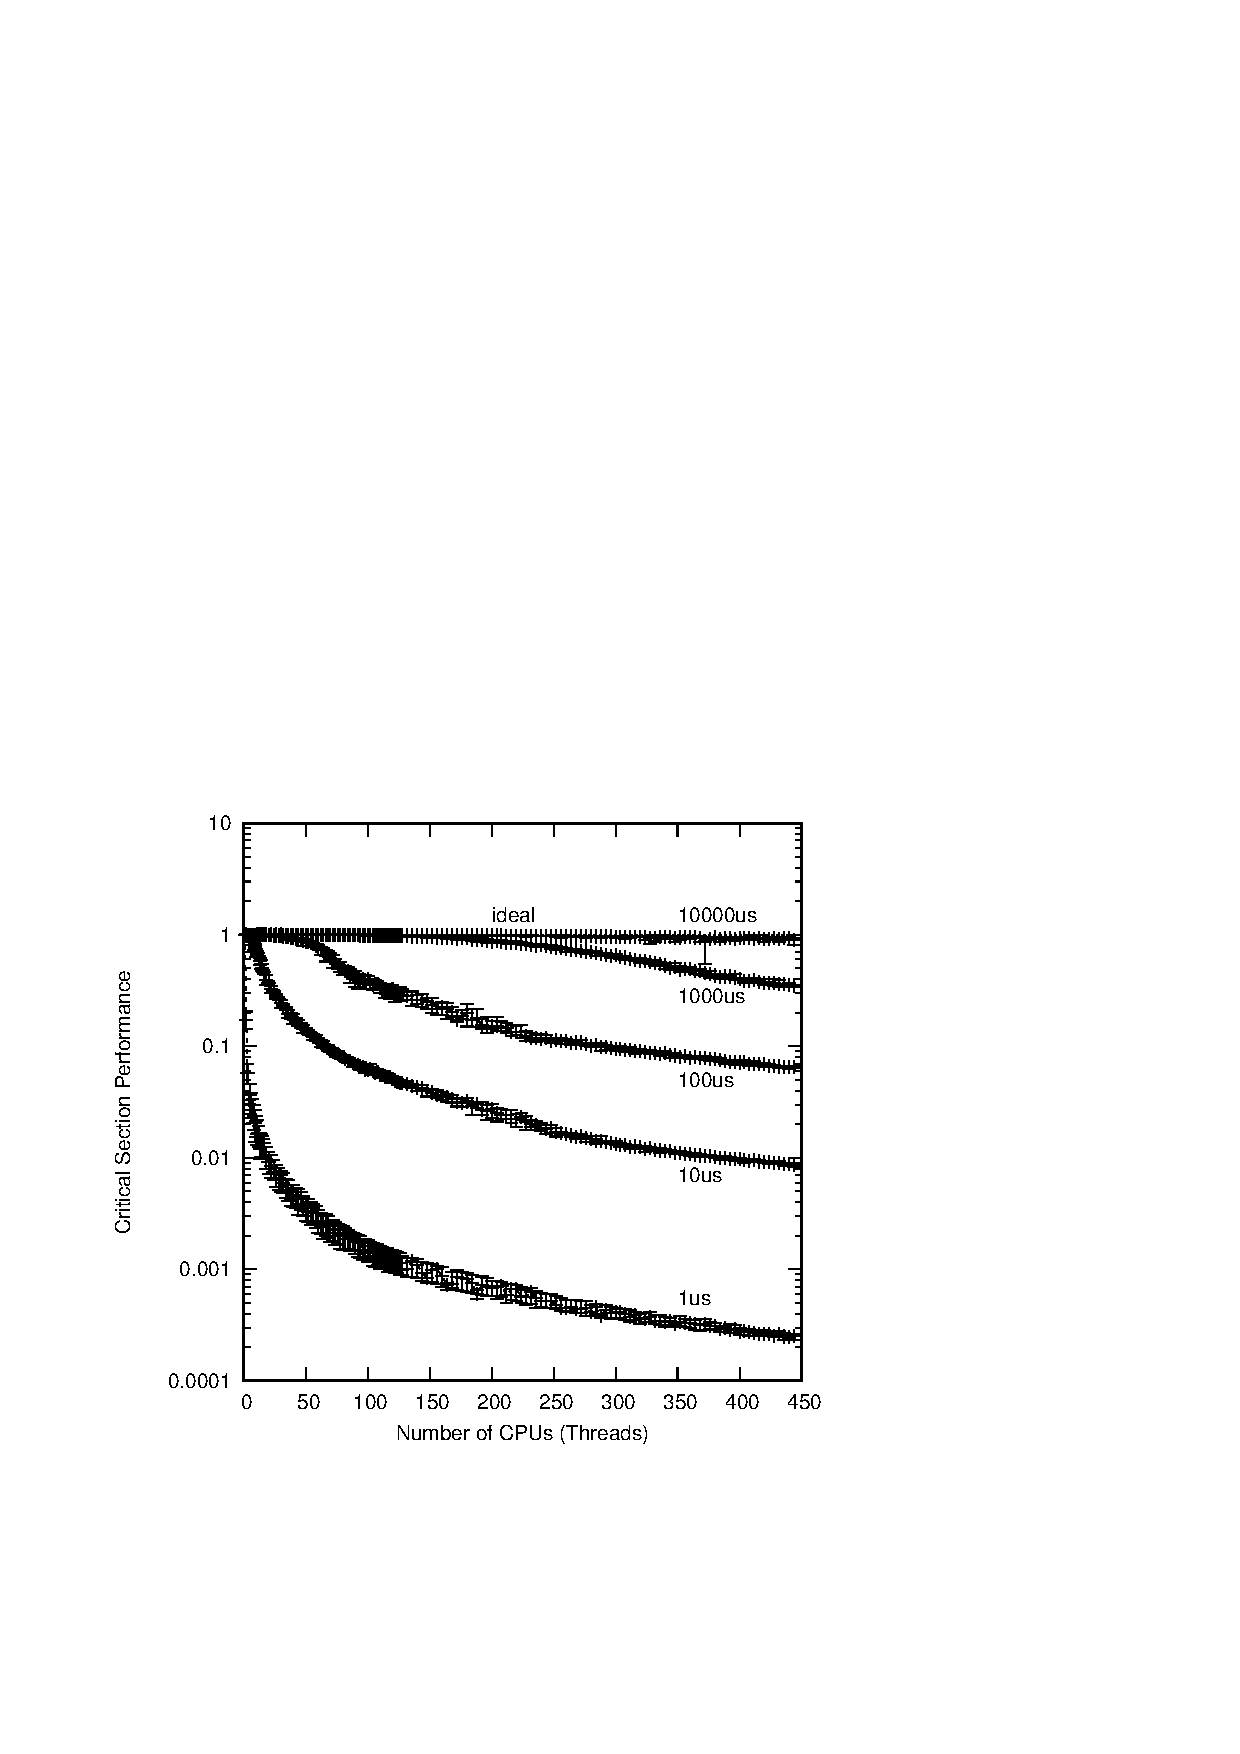
\includegraphics{CodeSamples/toolsoftrade/rwlockscale}}
\caption{Reader-Writer Lock Scalability vs. Microseconds in Critical Section on 8-Socket System With Intel Xeon Platinum 8176 CPUs @ 2.10GHz}
\label{fig:toolsoftrade:Reader-Writer Lock Scalability vs. Microseconds in Critical Section}
\end{figure}

Figure~\ref{fig:toolsoftrade:Reader-Writer Lock Scalability vs. Microseconds in Critical Section}
는 이 테스트를 224코어 Xeon 시스템에서 코어당 두개의 하드웨어 쓰레드를 사용해
총 448개의 소프트웨어에게 보이는 CPU 를 가지는 환경에서 수행되었을 때의 결과를
보입니다.
\co{thinktime} 패러미터는 모든 테스트 동안 0 이었으며, \co{holdtime} 패러미터는
1 마이크로세컨드부터 (그래프 상의 ``1us'') 10,000\,마이크로세컨드 (그래프 상의
``10000us'') 까지 적용되었습니다.
그려진 실제 값은 다음과 같습니다:
\begin{equation}
	\frac{L_N}{N L_1}
\end{equation}
여기서 $N$ 는 쓰레드의 수이며, $L_N$ 는 $N$ 개 쓰레드에 의한 락 획득 횟수이며
$L_1$ 는 단일 쓰레드에 의한 락 획득 횟수입니다.
이상적인 하드웨어와 소프트웨어 확장성 하에서는 이 값은 항상 1.0 이어야 합니다.

\iffalse

Figure~\ref{fig:toolsoftrade:Reader-Writer Lock Scalability vs. Microseconds in Critical Section}
shows the results of running this test on a 224-core Xeon system
with two hardware threads per core for a total of 448 software-visible
CPUs.
The \co{thinktime} parameter was zero for all these tests, and the
\co{holdtime} parameter set to values ranging from one microsecond (``1us''
on the graph) to 10,000\,microseconds (``10000us'' on the graph).
The actual value plotted is:
\begin{equation}
	\frac{L_N}{N L_1}
\end{equation}
where $N$ is the number of threads,
$L_N$ is the number of lock acquisitions by $N$ threads, and
$L_1$ is the number of lock acquisitions by a single thread.
Given ideal hardware and software scalability, this value will always
be 1.0.

\fi

그림 상에서 볼 수 있듯이, reader-writer 락킹의 확장성은 분명 이상적이지 않은데,
특히 작은 크기의 크리티컬 섹션에서 그렇습니다.
왜 읽기 락 획득이 그렇게 느린지 알아보기 위해선, 락을 획득하려는 모든 쓰레드가
\co{pthread_rwlock_t} 데이터 구조를 업데이트 한다는 걸 생각해 봅시다.
따라서, 만약 모든 448개의 쓰레드가 이 reader-writer 락을 동시에 읽기 모드로
획득하려 한다면, 이들은 \co{pthread_rwlock_t} 를 한번에 하나씩 업데이트 해야만
합니다.
운이 좋은 쓰레드는 거의 곧바로 그렇게 할 수 있겠지만, 가장 운이 나쁜 쓰레드는
다른 447개의 쓰레드가 업데이트를 끝낼 때까지 기다려야만 합니다.
이 상황은 CPU 를 추가할 수록 나빠지기만 할 겁니다.
그리고 y 축이 로그스케일이라는 점도 알아 두시기 바랍니다.
10,000\,마이크로세컨드의 기록이 상당히 이상적인 것으로 보이지만, 실제로는
이상적인 경우에 비해 10\,\% 뒤쳐집니다.

\iffalse

As can be seen in the figure, reader-writer locking scalability is
decidedly non-ideal, especially for smaller sizes of critical
sections.
To see why read-acquisition can be so slow, consider
that all the acquiring threads must update the \co{pthread_rwlock_t}
data structure.
Therefore, if all 448 executing threads attempt to
read-acquire the reader-writer lock concurrently, they must update
this underlying \co{pthread_rwlock_t} one at a time.
One lucky thread might do so almost immediately, but the least-lucky
thread must wait for all the other 447 threads to do their updates.
This situation will only get worse as you add CPUs.
Note also the logscale y-axis.
Even though the 10,000\,microsecond trace appears quite ideal, it has
in fact degraded by about 10\,\% from ideal.

\fi

\QuickQuizSeries{%
\QuickQuizB{
	단일 CPU 의 처리량과 비교하는 건 좀 너무한 거 아닌가요?

	\iffalse

	Isn't comparing against single-CPU throughput a bit harsh?

	\fi

}\QuickQuizAnswerB{
	전혀요.
	실제로, 이 비교는 무척 관대한 겁니다.
	좀 더 균형잡힌 비교는 락킹 기능이 제거된 상태에서의 단일 CPU 처리량에
	대한 것일 겁니다.

	\iffalse

	Not at all.
	In fact, this comparison was, if anything, overly lenient.
	A more balanced comparison would be against single-CPU
	throughput with the locking primitives commented out.

	\fi

}\QuickQuizEndB
%
\QuickQuizM{
	하지만 1마이크로세컨드는 크리티컬 섹션의 크기로 특별히 작은 건
	아닙니다.
	예를 들어 몇개의 명령만이 들어있는 것 같은, 훨씬 더 작은 크리티컬
	섹션이 필요할 땐 어떡해야 하죠?

	\iffalse

	But one microsecond is not a particularly small size for
	a critical section.
	What do I do if I need a much smaller critical section, for
	example, one containing only a few instructions?

	\fi

}\QuickQuizAnswerM{
	읽혀진 데이터가 \emph{절대} 바뀌지 않는다면, 그걸 접근하는 동안 어떤
	락도 잡고 있을 필요가 없습니다.
	해당 데이터가 충분히 가끔씩만 바뀐다면, 수행을 체크포인트하고, 모든
	쓰레드를 종료하고, 데이터를 변경한 후, 해당 체크포인트부터 재시작할 수
	있습니다.

	또다른 접근법은 쓰레드당 하나의 배타적 락을 두어서, 자신의 락을
	획득하는 것으로 거대한 reader-writer 락을 읽기 모드로 획득하게 하고,
	모든 쓰레드당 락을 획득하는 것으로 쓰기 모드 획득을 하도록 구현하는
	겁니다~\cite{WilsonCHsieh92a}.
	이는 읽기 쓰레드에게는 상당히 잘 동작하지만, 쓰기 쓰레드에게는 쓰레드의
	수가 늘어날수록 더 큰 오버헤드를 야기시킬 겁니다.

	매우 작은 크리티컬 섹션을 처리하는 다른 효율적 방법들이
	Chapter~\ref{chp:Deferred Processing} 에 설명되어 있습니다.

	\iffalse

	If the data being read \emph{never} changes, then you do not
	need to hold any locks while accessing it.
	If the data changes sufficiently infrequently, you might be
	able to checkpoint execution, terminate all threads, change
	the data, then restart at the checkpoint.

	Another approach is to keep a single exclusive lock per
	thread, so that a thread read-acquires the larger aggregate
	reader-writer lock by acquiring its own lock, and write-acquires
	by acquiring all the per-thread locks~\cite{WilsonCHsieh92a}.
	This can work quite well for readers, but causes writers
	to incur increasingly large overheads as the number of threads
	increases.

	Some other ways of efficiently handling very small critical
	sections are described in Chapter~\ref{chp:Deferred Processing}.

	\fi

}\QuickQuizEndM
%
\QuickQuizM{
	여기 사용된 시스템은 몇년 이상 되었고, 새로운 하드웨어는 더 빠를
	겁니다.
	그러니 누가 reader-writer 락이 느려짐에 대해 걱정하겠습니까?

	\iffalse

	The system used is a few years old, and new hardware should
	be faster.
	So why should anyone worry about reader-writer locks being slow?

	\fi

}\QuickQuizAnswerE{
	일반적으로 새로운 하드웨어는 개선됩니다.
	하지만, reader-writer 락이 448 CPU 에서 이상적 성능을 내게끔 하기
	위해선 수천수만배의 개선을 필요로 할 겁니다.
	더 나쁜 것이, CPU 의 갯수가 늘어날수록 필요한 성능 향상이 더 커집니다.
	따라서 reader-writer 락킹의 성능 문제는 상당한 시간 동안 우리 곁에 있을
	겁니다.

	\iffalse

	In general, newer hardware is improving.
	However, it will need to improve several orders of magnitude
	to permit reader-writer lock to achieve ideal performance on
	448 CPUs.
	Worse yet, the greater the number of CPUs, the larger the
	required performance improvement.
	The performance problems of reader-writer locking are therefore
	very likely to be with us for quite some time to come.

	\fi

}\QuickQuizEndE
}

이런 제한에도 불구하고, reader-writer 락킹은 많은 경우에 유용한데, 예를 들어
읽기 쓰레드들이 응답시간이 긴 파일이나 네트워크 I/O 를 처리해야 하는
경우입니다.
일부 대안도 존재하는데,
Chapter~\ref{chp:Counting} 와~\ref{chp:Deferred Processing} 에서 보입니다.

\iffalse

Despite these limitations, reader-writer locking is quite useful in many
cases, for example when the readers must do high-latency file or network I/O\@.
There are alternatives, some of which will be presented in
Chapters~\ref{chp:Counting} and \ref{chp:Deferred Processing}.

\fi

\subsection{Atomic Operations (\GCC\ Classic)}
\label{sec:toolsoftrade:Atomic Operations (gcc Classic)}

Figure~\ref{fig:toolsoftrade:Reader-Writer Lock Scalability vs. Microseconds in Critical Section}
는 reader-writer 락킹의 오버헤드는 가장 작은 크리티컬 섹션에서 가장 심각함을
보이며, 따라서 작은 크리티컬 섹션들을 보호하는 어떤 다른 방법이 있다면 좋을
겁니다.
그런 한가지 방법은 어토믹 오퍼레이션입니다.
\begin{fcvref}[ln:toolsoftrade:rwlockscale:reader:reader]
우린 이미 하나의 어토믹 오퍼레이션을 봤는데,
Listing~\ref{lst:toolsoftrade:Measuring Reader-Writer Lock Scalability}
의 \clnref{atmc_inc} 의 \apig{__sync_fetch_and_add()} 기능입니다.
이 기능은 두번째 인자의 값을 첫번째 인자로 참조되는 값에 원자적으로 더하고 기존
값을 리턴합니다 (이 경우엔 무시되었습니다).
한쌍의 쓰레드가 동시에 같은 변수에 대해 \co{__sync_fetch_and_add()} 를 실행하면
이 변수의 결과값은 두 더하기의 결과를 포함하게 됩니다.
\end{fcvref}

\iffalse

Figure~\ref{fig:toolsoftrade:Reader-Writer Lock Scalability vs. Microseconds in Critical Section}
shows that the overhead of reader-writer locking is most severe for the
smallest critical sections, so it would be nice to have some other way
of protecting tiny critical sections.
One such way uses atomic operations.
\begin{fcvref}[ln:toolsoftrade:rwlockscale:reader:reader]
We have seen an atomic operation already, namely the
\apig{__sync_fetch_and_add()} primitive on \clnref{atmc_inc} of
Listing~\ref{lst:toolsoftrade:Measuring Reader-Writer Lock Scalability}.
This primitive atomically adds the value of its second argument to
the value referenced by its first argument, returning the old value
(which was ignored in this case).
If a pair of threads concurrently execute \co{__sync_fetch_and_add()} on
the same variable, the resulting value of the variable will include
the result of both additions.
\end{fcvref}

\fi

\GNUC\ 컴파일러는
 \apig{__sync_fetch_and_sub()},
\apig{__sync_fetch_and_or()},
\apig{__sync_fetch_and_and()},
\apig{__sync_fetch_and_xor()}, 그리고
\apig{__sync_fetch_and_nand()}
를 포함한 수많은 추가적 어토믹 오퍼레이션을 제공하는데, 이것들은 모두 기존 값을
리턴합니다.
그대신 새 값이 필요하다면,
\apig{__sync_add_and_fetch()},
\apig{__sync_sub_and_fetch()},
\apig{__sync_or_and_fetch()},
\apig{__sync_and_and_fetch()},
\apig{__sync_xor_and_fetch()}, 그리고
\apig{__sync_nand_and_fetch()}
기능을 사용할 수 있습니다.

\iffalse

The \GNUC\ compiler offers a number of additional atomic operations,
including \apig{__sync_fetch_and_sub()},
\apig{__sync_fetch_and_or()},
\apig{__sync_fetch_and_and()},
\apig{__sync_fetch_and_xor()}, and
\apig{__sync_fetch_and_nand()}, all of which return the old value.
If you instead need the new value, you can instead use the
\apig{__sync_add_and_fetch()},
\apig{__sync_sub_and_fetch()},
\apig{__sync_or_and_fetch()},
\apig{__sync_and_and_fetch()},
\apig{__sync_xor_and_fetch()}, and
\apig{__sync_nand_and_fetch()} primitives.

\fi

\QuickQuiz{
	그런 두 종류의 기능이 정말로 필요한가요?

	\iffalse

	Is it really necessary to have both sets of primitives?

	\fi

}\QuickQuizAnswer{
	엄밀히 말하면, 필요 없습니다.
	두번째 집합의 어느 것이든 그에 연관된 첫번째 집합 내의 것을 사용해
	구현될 수 있습니다.
	예를 들어, \apig{__sync_nand_and_fetch()} 를 다음과 같이
	\apig{__sync_fetch_and_nand()} 로 구현할 수 있습니다.

	\iffalse

	Strictly speaking, no.
	One could implement any member of the second set using the
	corresponding member of the first set.
	For example, one could implement \apig{__sync_nand_and_fetch()}
	in terms of \apig{__sync_fetch_and_nand()} as follows:

	\fi

\begin{VerbatimU}
tmp = v;
ret = __sync_fetch_and_nand(p, tmp);
ret = ~ret & tmp;
\end{VerbatimU}

	비슷하게 \apig{__sync_fetch_and_add()},
	\apig{__sync_fetch_and_sub()}, 그리고 \apig{__sync_fetch_and_xor()}
	를 나중값을 리턴하는 것들을 이용해 구현할 수도 있습니다.

	하지만, 그 대안인 앞의 형태가 프로그래머에게도 컴파일러/라이브러리
	구현자에게도 상당히 편리할 수 있습니다.

	\iffalse

	It is similarly possible to implement \apig{__sync_fetch_and_add()},
	\apig{__sync_fetch_and_sub()}, and \apig{__sync_fetch_and_xor()}
	in terms of their post-value counterparts.

	However, the alternative forms can be quite convenient, both
	for the programmer and for the compiler/library implementor.

	\fi

}\QuickQuizEnd

고전적인 compare-and-swap 오퍼레이션은 \apig{__sync_bool_compare_and_swap()} 와
\apig{__sync_val_compare_and_swap()}, 한쌍의 기능들로 제공됩니다.
이 기능들 둘 모두 새로운 값을 원자적으로 업데이트 합니다만 그 기존 값이 명시된
이전 값과 동일할 때만 그렇습니다.
앞의 첫번째 변종은 이 오퍼레이션이 성공하면 1 을, 실패하면 0 을 리턴하는데,
예를 들어 그 기존 값이 명시된 이전 값과 갖지 않은 경우 실패합니다.
두번째 변종은 해당 위치의 기존값을 리턴하는데, 즉, 이 값이 명시된 이전 값과
동일하다면 이 오퍼레이션은 성공했음을 의미합니다.
모든 단일 위치로의 어토믹 오퍼레이션은 앞의 오퍼레이션들이 종종 더
효율적이지만, compare-and-swap 을 이용해 구현될 수 있다는 점에서
compare-and-swap 오퍼레이션은 ``보편적'' 입니다.
이 compare-and-swap 오퍼레이션은 더 다양한 어토믹 오퍼레이션 집합의 기본으로
사용될 수도 있습니다만, 이것들을 더 다듬는 것은 종종 복잡도, 확장성, 성능
문제로 고통받습니다~\cite{MauriceHerlihy90a}.

\iffalse

The classic compare-and-swap operation is provided by a pair of
primitives, \apig{__sync_bool_compare_and_swap()} and
\apig{__sync_val_compare_and_swap()}.
Both of these primitives atomically update a location to a new value,
but only if its prior value was equal to the specified old value.
The first variant returns 1 if the operation succeeded and 0 if it
failed, for example, if the prior value was not equal to the specified
old value.
The second variant returns the prior value of the location, which, if
equal to the specified old value, indicates that the operation succeeded.
Either of the compare-and-swap operation is ``universal'' in the sense
that any atomic operation on a single location can be implemented in
terms of compare-and-swap, though the earlier operations are often
more efficient where they apply.
The compare-and-swap operation is also capable of serving as the basis
for a wider set of atomic operations, though the more elaborate of
these often suffer from complexity, scalability, and performance
problems~\cite{MauriceHerlihy90a}.

\fi

\QuickQuiz{
	이 어토믹 오퍼레이션들은 밑바닥의 인스트럭션 셋을 이용해 직접적으로
	지원되는 단일 어토믹 인스트럭션을 생성하는 경우가 많을 텐데, 그것이
	일을 하는데 가장 빠른 방법일까요?

	\iffalse

	Given that these atomic operations will often be able to
	generate single atomic instructions that are directly
	supported by the underlying instruction set, shouldn't
	they be the fastest possible way to get things done?

	\fi

}\QuickQuizAnswer{
	불행히도, 그렇지 않습니다.
	극명한 반대 예제를 위해선 Chapter~\ref{chp:Counting} 를 읽어보시기
	바랍니다.

	\iffalse

	Unfortunately, no.
	See Chapter~\ref{chp:Counting} for some stark counterexamples.

	\fi

}\QuickQuizEnd

\apig{__sync_synchronize()} 기능은 컴파일러와 CPU 모두 오퍼레이션을 재배치하지
못하게 하는 ``메모리 배리어'' 를 수행하는데,
Chapter~\ref{chp:Advanced Synchronization: Memory Ordering}
에서 이야기 합니다.
어떤 경우에는 컴파일러의 오퍼레이션 재배치 기능은 제한하지만 CPU 는 내버려 둬도
충분한데, 그런 때에는 \apik{barrier()} 기능이 사용될 수 있습니다.
\begin{fcvref}[ln:toolsoftrade:lock:reader_writer:reader]
어떤 경우에는 컴파일러가 특정 메모리 읽기를 최적화를 위해 없애버리는 것을 막을
필요가 있는데, 그럴 때에는
Listing~\ref{lst:toolsoftrade:Demonstration of Exclusive Locks}
의 \clnref{read_x} 에서와 같이 \apik{READ_ONCE()} 기능이 사용될 수 있습니다.
\end{fcvref}
비슷하게, \apik{WRITE_ONCE()} 기능은 컴파일러가 특정 메모리 쓰기를 최적화해
없애버리는 걸 막는데 사용될 수 있습니다.
이 마지막 세개의 기능들은 \GCC 에서 직접 제공되진 않습니다만
Listing~\ref{lst:toolsoftrade:Compiler Barrier Primitive (for GCC)}
에 보인 것처럼 간단히 구현될 수 있으며, 이 세가지가
Section~\ref{sec:toolsoftrade:Accessing Shared Variables}
에서 길게 설명됩니다.
대안적으로, \apialtk{READ_ONCE(x)}{READ_ONCE()} 가 \GCC\ 내재 기능인 
\apialtg{__atomic_load_n(&x, __ATOMIC_RELAXED)}{__atomic_load_n()}
와 공통되는 부분이 많으며, \apik{WRITE_ONCE()} 는 \GCC\ 내재 기능인
\apialtg{__atomic_store_n(&x, v, __ATOMIC_RELAXED)}{__atomic_store_n()} 와
공통되는 부분이 많습니다.

\iffalse

The \apig{__sync_synchronize()} primitive issues a ``memory barrier'',
which constrains both the compiler's and the CPU's ability to reorder
operations, as discussed in
Chapter~\ref{chp:Advanced Synchronization: Memory Ordering}.
In some cases, it is sufficient to constrain the compiler's ability
to reorder operations, while allowing the CPU free rein, in which
case the \apik{barrier()} primitive may be used.
\begin{fcvref}[ln:toolsoftrade:lock:reader_writer:reader]
In some cases, it is only necessary to ensure that the compiler
avoids optimizing away a given memory read, in which case the
\apik{READ_ONCE()} primitive may be used, as it was on \clnref{read_x} of
Listing~\ref{lst:toolsoftrade:Demonstration of Exclusive Locks}.
\end{fcvref}
Similarly, the \apik{WRITE_ONCE()} primitive may be used to prevent the
compiler from optimizing away a given memory write.
These last three primitives are not provided directly by \GCC,
but may be implemented straightforwardly as shown in
Listing~\ref{lst:toolsoftrade:Compiler Barrier Primitive (for GCC)},
and all three are discussed at length in
Section~\ref{sec:toolsoftrade:Accessing Shared Variables}.
Alternatively, \apialtk{READ_ONCE(x)}{READ_ONCE()} has much in common with
the \GCC\  intrinsic
\apialtg{__atomic_load_n(&x, __ATOMIC_RELAXED)}{__atomic_load_n()}
and \apik{WRITE_ONCE()} has much in common with the \GCC\ 
intrinsic \apialtg{__atomic_store_n(&x, v, __ATOMIC_RELAXED)}{__atomic_store_n()}.

\fi

\begin{listing}[tb]
\input{CodeSamples/api-pthreads/api-pthreads@compiler_barrier.fcv}
\caption{Compiler Barrier Primitive (for \GCC)}
\label{lst:toolsoftrade:Compiler Barrier Primitive (for GCC)}
\end{listing}

\QuickQuiz{
	\apikh{ACCESS_ONCE()} 에는 무슨 일이 벌어진 건가요?

	\iffalse

	What happened to \apikh{ACCESS_ONCE()}?

	\fi

}\QuickQuizAnswer{
	2018년 v4.15 릴리즈에서, 리눅스 커널의 \apikh{ACCESS_ONCE()} 는 읽기와
	쓰기를 위해 각각 \apik{READ_ONCE()} 와 \apik{WRITE_ONCE()} 로
	교체되었습니다~\cite{JonCorbet2012ACCESS:ONCE,
	JonathanCorbet2014ACCESS:ONCEcompilerBugs,
	MarkRutland2017ACCESS:ONCE:remove}.
	\apikh{ACCESS_ONCE()} 는 RCU 코드에 사용되기 위해 만들어졌습니다만, 곧
	코어 API 가 되었습니다~\cite{
	PaulEMcKenney2007ACCESS:ONCE:rcu,
	LinusTorvalds2008ACCESS:ONCE:move}.
	리눅스 커널의 \apik{READ_ONCE()} 와 \apik{WRITE_ONCE()} 는 원래의
	\apikh{ACCESS_ONCE()} 구현과는 상당히 다른 복잡한 형태로 진화했는데 큰
	구조체에도 access-once 기능을 지원하지만 해당 구조체가 하나의 기계
	명령어로 로드되고 스토어 될 수 없을 때 로드/스토어가 찢겨지는 가능성을
	막기 위해서였습니다.

	\iffalse

	In the 2018 v4.15 release, the Linux kernel's \apikh{ACCESS_ONCE()} was
	replaced by \apik{READ_ONCE()} and \apik{WRITE_ONCE()} for reads and
	writes, respectively~\cite{JonCorbet2012ACCESS:ONCE,
	JonathanCorbet2014ACCESS:ONCEcompilerBugs,
	MarkRutland2017ACCESS:ONCE:remove}.
	\apikh{ACCESS_ONCE()} was introduced as a helper in RCU code, but was
	promoted to core API soon afterward~\cite{
	PaulEMcKenney2007ACCESS:ONCE:rcu,
	LinusTorvalds2008ACCESS:ONCE:move}.
	Linux kernel's \apik{READ_ONCE()} and \apik{WRITE_ONCE()} have
	evolved into complex forms that look quite different than
	the original \apikh{ACCESS_ONCE()} implementation due to the
	need to support access-once semantics for large structures,
	but with the possibility of load/store tearing if the structure
	cannot be loaded and stored with a single machine instruction.

	\fi

}\QuickQuizEnd

\subsection{Atomic Operations (C11)}
\label{sec:toolsoftrade:Atomic Operations (C11)}

C11 표준은 로드 (\apic{atomic_load()}), 스토어 (\apic{atomic_store()}), 메모리
배리어 (\apic{atomic_thread_fence()} 와 \apic{atomic_signal_fence()}), 그리고
read-modify-write 어토믹 오퍼레이션들을 포함한 어토믹 오퍼레이션들을
추가했습니다.
이 read-modify-write 어토믹 오퍼레이션에는
\apic{atomic_fetch_add()},
\apic{atomic_fetch_sub()},
\apic{atomic_fetch_and()},
\apic{atomic_fetch_xor()},
\apic{atomic_exchange()},
\apic{atomic_compare_exchange_strong()},
그리고
\apic{atomic_compare_exchange_weak()}
이 포함됩니다.
이것들은
Section~\ref{sec:toolsoftrade:Atomic Operations (gcc Classic)}
에서 설명한 것들과 비슷하게 동작합니다만 모든 오퍼레이션의 \co{_explicit}
변종의 추가된 메모리 순서 인자와 함께 동작합니다.
메모리 순서 인자가 없이는 이 모든 어토믹오퍼레이션이 완전한 순서규칙 (fully
ordered) 아래 동작하며, 이 인자가 주어지면 좀 더 약한 순서규칙 (weaker
ordering) 을 허용합니다.
예를 들어, ``\apialtc{atomic_load_explicit(&a, memory_order_relaxed)}
{atomic_load_explicit()}'' 는 대략적으로 말해서 리눅스 커널의
``\apik{READ_ONCE()}'' 와 비슷합니다.\footnote{
	메모리 순서 규칙은
	Chapter~\ref{chp:Advanced Synchronization: Memory Ordering} 와
	Appendix~\ref{chp:app:whymb:Why Memory Barriers?}
	에 더 자세히 설명되어 있습니다.}

\iffalse

The C11 standard added atomic operations,
including loads (\apic{atomic_load()}),
stores (\apic{atomic_store()}),
memory barriers (\apic{atomic_thread_fence()} and
\apic{atomic_signal_fence()}), and read-modify-write atomics.
The read-modify-write atomics include
\apic{atomic_fetch_add()},
\apic{atomic_fetch_sub()},
\apic{atomic_fetch_and()},
\apic{atomic_fetch_xor()},
\apic{atomic_exchange()},
\apic{atomic_compare_exchange_strong()},
and
\apic{atomic_compare_exchange_weak()}.
These operate in a manner similar to those described in
Section~\ref{sec:toolsoftrade:Atomic Operations (gcc Classic)},
but with the addition of memory-order arguments to \co{_explicit}
variants of all of the operations.
Without memory-order arguments, all the atomic operations are
fully ordered, and the arguments permit weaker orderings.
For example, ``\apialtc{atomic_load_explicit(&a, memory_order_relaxed)}
{atomic_load_explicit()}''
is vaguely similar to the Linux kernel's ``\apik{READ_ONCE()}''.\footnote{
	Memory ordering is described in more detail in
	Chapter~\ref{chp:Advanced Synchronization: Memory Ordering} and
	Appendix~\ref{chp:app:whymb:Why Memory Barriers?}.}

\fi

\subsection{Atomic Operations (Modern \GCC)}
\label{sec:toolsoftrade:Atomic Operations (Modern gcc)}

C11 어토믹 오퍼레이션의 한계점 중 하나는 특수한 어토믹 타입에만 그것들이 적용될
수 있다는 것으로, 이는 문제가 될 수 있습니다.
따라서 \GNUC\ 컴파일러는 어토믹 내재기능들을 제공하는데,
\apig{__atomic_load()},
\apig{__atomic_load_n()},
\apig{__atomic_store()},
\apig{__atomic_store_n()},
\apig{__atomic_thread_fence()} 등이 포함됩니다.
이 내재기능들은 C11 의 비슷한 것들과 같은 기능을 제공합니다만, 평범한 어토믹
타입이 아닌 객체들에도 사용될 수 있습니다.
이것들 중 일부는 아래 리스트 중 하나의 메모리 순서 인자를 받을 수 있습니다:
\apig{__ATOMIC_RELAXED},
\apig{__ATOMIC_CONSUME},
\apig{__ATOMIC_ACQUIRE},
\apig{__ATOMIC_RELEASE},
\apig{__ATOMIC_ACQ_REL}, 그리고
\apig{__ATOMIC_SEQ_CST}.

\iffalse

One restriction of the C11 atomics is that they apply only to special
atomic types, which can be problematic.
The \GNUC\ compiler therefore provides atomic intrinsics, including
\apig{__atomic_load()},
\apig{__atomic_load_n()},
\apig{__atomic_store()},
\apig{__atomic_store_n()},
\apig{__atomic_thread_fence()}, etc.
These intrinsics offer the same semantics as their C11 counterparts,
but may be used on plain non-atomic objects.
Some of these intrinsics may be passed a memory-order argument from
this list:
\apig{__ATOMIC_RELAXED},
\apig{__ATOMIC_CONSUME},
\apig{__ATOMIC_ACQUIRE},
\apig{__ATOMIC_RELEASE},
\apig{__ATOMIC_ACQ_REL}, and
\apig{__ATOMIC_SEQ_CST}.

\fi

\subsection{Per-Thread Variables}
\label{sec:toolsoftrade:Per-Thread Variables}

Thread-specific data, thread-local storage, 또는 다른 덜 겸손한 이름으로도
불리는 쓰레드별 변수 (per-thread variables) 는 동시성 코드에서 굉장히 자주
사용되는데
Chapter~\ref{chp:Counting} and~\ref{chp:Data Ownership} 에서 더 이야기 될
겁니다.
POSIX 는 쓰레드별 변수 생성을 (그리고 그에 연관된 키를 리턴하기 위해) 위해
\apipx{pthread_key_create()} 를, 키에 연관된 쓰레드별 변수의 삭제를 위해
\apipx{pthread_key_delete()} 를, 현재 쓰레드의 특정 키에 연관된 변수의 값을
설정하기 위해 \apipx{pthread_setspecific()} 를, 이 값을 리턴하기 위해
\apipx{pthread_getspecific()} 을 제공합니다.

\iffalse

Per-thread variables, also called thread-specific data, thread-local
storage, and other less-polite names, are used extremely
heavily in concurrent code, as will be explored in
Chapters~\ref{chp:Counting} and~\ref{chp:Data Ownership}.
POSIX supplies the \apipx{pthread_key_create()} function to create a
per-thread variable (and return the corresponding key),
\apipx{pthread_key_delete()} to delete the per-thread variable corresponding
to key,
\apipx{pthread_setspecific()} to set the value of the current thread's
variable corresponding to the specified key,
and \apipx{pthread_getspecific()} to return that value.

\fi

여러 컴파일러가 (\GCC 포함) 해당 변수가 쓰레드별로 되어야 함을 나타내기 위해
변수 정의 부분에 사용될 수 있는 \apig{__thread} 지시어를 제공합니다.
그러면 이 변수의 이름은 그 변수의 현재 쓰레드의 값을 평범하게 접근하는데 사용될
수 있습니다.
물론, \apig{__thread} 는 POSIX thread-specific 데이터보다 사용하기가 훨씬 쉽고,
때문에 \GCC\ 또는 \co{__thread} 를 지원하는 컴파일러로만 빌드되는 코드에서는 더
선호되는 편입니다.

다행히도, C11 표준은 \apig{__thread} 의 자리에 사용될 수 있는
\apic{_Thread_local} 키워드를 도입했습니다.
충분한 시간이 지난 후에는 이 새로운 키워드가 \co{__thread} 의 좋은 사용성과
POSIX thread-specific data 의 이식성을 결합시킬 겁니다.

\iffalse

A number of compilers (including \GCC) provide a \apig{__thread} specifier
that may be used in a variable definition to designate that variable
as being per-thread.
The name of the variable may then be used normally to access the
value of the current thread's instance of that variable.
Of course, \apig{__thread} is much easier to use than the POSIX
thead-specific data, and so \co{__thread} is usually preferred for
code that is to be built only with \GCC\ or other compilers supporting
\co{__thread}.

Fortunately, the C11 standard introduced a \apic{_Thread_local} keyword
that can be used in place of \apig{__thread}.
In the fullness of time, this new keyword should combine the ease of use
of \co{__thread} with the portability of POSIX thread-specific data.

\fi

\section{Alternatives to POSIX Operations}
\label{sec:toolsoftrade:Alternatives to POSIX Operations}
%
\epigraph{The strategic marketing paradigm of Open Source is a massively
	  parallel drunkard's walk filtered by a Darwinistic process.}
	 {\emph{Bruce Perens}}

불행히도, 쓰레드 오퍼레이션, 락킹 기능, 그리고 어토믹 오퍼레이션은 다양한 표준
위원회들이 그것들에 다가가기 훨씬 전부터 사용되어왔습니다.
그 결과, 이 오퍼레이션들이 어떻게 지원되는지에 대한 상당한 차이들이 존재합니다.
역사적인 이유로, 또는 특정 환경에서의 더 나은 성능을 위해서 이 오퍼레이션들이
어셈블리 언어로 구현되는 경우는 상당히 흔합니다.
예를 들어, \GCC 의 \co{__sync_} 기능군은 모두 완전한 메모리 순서 규칙을
제공하는데, 이는 과거에 많은 개발자들을 완전한 메모리 순서 규칙이 필요하지 않은
상황을 위한 각자의 구현을 만들게 이끌었습니다.
다음 섹션들은 리눅스 커널의 일부 대안과 이 책의 예제 코드에서 사용된 역사적
기능들을 보입니다.

\iffalse

Unfortunately, threading operations, locking primitives, and atomic
operations were in reasonably wide use long before the various standards
committees got around to them.
As a result, there is considerable variation in how these operations
are supported.
It is still quite common to find these operations implemented in
assembly language, either for historical reasons or to obtain better
performance in specialized circumstances.
For example, \GCC's \co{__sync_} family of primitives all provide full
memory-ordering semantics, which in the past motivated many developers
to create their own implementations for situations where the full memory
ordering semantics are not required.
The following sections show some alternatives from the Linux kernel
and some historical primitives used by this book's sample code.

\fi

\subsection{Organization and Initialization}
\label{sec:toolsoftrade:Organization and Initialization}

많은 환경이 특별한 초기화 코드를 필요로 하지 않지만, 이 책의 예제 코드는
\apipx{pthread_t} 에서 연속된 정수들로의 매핑을초기화 하는 \apipf{smp_init()}
를 호출하는 것으로 시작합니다.
유저스페이스 RCU 라이브러리\footnote{
	RCU 에 대한 더 많은 정보를 위해선
	\cref{sec:defer:Read-Copy Update (RCU)} 를 보시기 바랍니다.}
역시 비슷하게 \apiur{rcu_init()} 호출을 필요로 합니다.
생성자를 지원하는 환경 (\GCC 의 것 같은) 에서는 이 호출들이 숨겨질 수 있지만,
유저스페이스 RCU 라이브러리에서 지원되는 대부분의 RCU 변종들은 각 쓰레드가
쓰레드 생성 시에 \apiur{rcu_register_thread()} 를, 쓰레드 종료 전에
\apiur{rcu_unregister_thread()} 를 호출할 것을 필요로 합니다.

리눅스 커널의 경우, 커널은 특수한 초기화 코드 호출을 필요로 하지 않는다고
봐야할지 또는 커널의 부팅 시의 코드가 사실은 필요한 초기화 코드라고 봐야할지에
대한 것은 철학적 질문입니다.

\iffalse

Although many environments do not require any special initialization
code, the code samples in this book start with a call to \apipf{smp_init()},
which initializes a mapping from \apipx{pthread_t} to consecutive integers.
The userspace RCU library\footnote{
	See \cref{sec:defer:Read-Copy Update (RCU)} for more information
	on RCU\@.}
similarly requires a call to \apiur{rcu_init()}.
Although these calls can be hidden in environments (such as that of
\GCC) that support constructors,
most of the RCU flavors supported by the userspace RCU library
also require each thread invoke \apiur{rcu_register_thread()} upon thread
creation and \apiur{rcu_unregister_thread()} before thread exit.

In the case of the Linux kernel, it is a philosophical question as to
whether the kernel does not require calls to special initialization
code or whether the kernel's boot-time code is in fact the required
initialization code.

\fi

\subsection{Thread Creation, Destruction, and Control}
\label{sec:toolsoftrade:Thread Creation, Destruction, and Control}

리눅스 커널은 kthread를 추적하기 위해 \apik{struct task_struct} 포인터를,
그것들을 생성하기 위해 \apik{kthread_create()} 를, 명시적으로 멈출 것을
제안하기 위해 (POSIX 에는 비슷한 게 없습니다) \apik{kthread_should_stop()}
을,\footnote{
	POSIX 환경에서는 \apik{kthread_should_stop()} 의 부재를 해결하기 위해
	\co{pthread_join()} 과 함께 제대로 동기화 되는 boolean 플래그를 사용할
	수 있습니다.}
그것들이 멈추기를 기다리기 위해 \apik{kthread_stop()} 을, 그리고 시간제한을 둔
기다림을 위해 \apik{schedule_timeout_interruptible()} 을 사용합니다.
몇가지 추가적인 kthread 관리 API 가 존재합니다만, 이것들만으로도 좋은 시작 내지
검색어가 될 수 있습니다.

CodeSamples API 는 제어의 장소인 ``threads'' 에 집중합니다.\footnote{
	비슷한 소프트웨어의 것들을 위한 많은 다른 이름들이 있는데 ``프로세스'',
	``태스크'', ``파이버'', ``이벤트'', ``수행 에이전트'' 등이 있습니다.
	비슷한 설계 원칙이 이것들 모두에 적용됩니다.}
그런 쓰레드 각각은 \apipf{thread_id_t} 타입의 식별자를 가지며 동시에 수행 되는
두개의 쓰레드가 같은 지시어를 갖지는 못합니다.
쓰레드는 쓰레드별 지역 상태를 제외한 모든 것을 공유하는데\footnote{
	순환적 정의에서는 이게 어떻게 될까요?}
프로그램 카운터와 스택이 포함됩니다.

\iffalse

The Linux kernel uses
\apik{struct task_struct} pointers to track kthreads,
\apik{kthread_create()} to create them,
\apik{kthread_should_stop()} to externally suggest that they stop
(which has no POSIX equivalent),\footnote{
	POSIX environments can work around the lack of
	\apik{kthread_should_stop()} by using a properly synchronized
	boolean flag in conjunction with \co{pthread_join()}.}
\apik{kthread_stop()} to wait for them to stop, and
\apik{schedule_timeout_interruptible()} for a timed wait.
There are quite a few additional kthread-management APIs, but this
provides a good start, as well as good search terms.

The CodeSamples API focuses on ``threads'', which are a locus of
control.\footnote{
	There are many other names for similar software constructs, including
	``process'', ``task'', ``fiber'', ``event'', ``execution agent'',
	and so on.
	Similar design principles apply to all of them.}
Each such thread has an identifier of type \apipf{thread_id_t},
and no two threads running at a given time will have the same
identifier.
Threads share everything except for per-thread local state,\footnote{
	How is that for a circular definition?}
which includes program counter and stack.

\fi

Listing~\ref{lst:toolsoftrade:Thread API} 에 쓰레드 API 가 보여져 있으며, 그
멤버들이 다음 섹션에서 설명됩니다.

\iffalse

The thread API is shown in
Listing~\ref{lst:toolsoftrade:Thread API}, and members are described in the
following sections.

\fi

\begin{listing}[tbp]
\begin{VerbatimL}[numbers=none,xleftmargin=2pt]
int smp_thread_id(void)
thread_id_t create_thread(void *(*func)(void *), void *arg)
for_each_thread(t)
for_each_running_thread(t)
void *wait_thread(thread_id_t tid)
void wait_all_threads(void)
\end{VerbatimL}
\caption{Thread API}
\label{lst:toolsoftrade:Thread API}
\end{listing}

\subsubsection{\tco{create_thread()}}

\apipf{create_thread()} 기능은 새로운 쓰레드를 하나 생성하고,
\apipf{create_thread()} 의 첫번째 인자로 명시된 \co{func} 함수에서 이 새
쓰레드의 수행을 시작하며, \apipf{create_thread()} 의 두번째 인자로 명시된
인자를 넘겨줍니다.
이 새로 생성된 쓰레드는 \co{func} 로 명시된 시작 함수가 리턴할 때 종료됩니다.
\apipf{create_thread()} 기능은 새로 생성된 자식 쓰레드에 연관된
\apipf{thread_id_t} 를 리턴합니다.

이 기능은 해당 프로그램이 생성한 쓰레드의 수를 암묵적으로 세면서
\apipf{NR_THREADS} 보다 많은 수의 쓰레드가 생성되면 프로그램을 종료시킵니다.
\apipf{NR_THREADS} 는 컴파일 시점에 변경될 수 있는 상수입니다만 일부 시스템은
허용 가능한 쓰레드의 수에 대한 상한선을 가지고 있을 수도 있습니다.

\iffalse

The \apipf{create_thread()} primitive creates a new thread,
starting the new thread's execution
at the function \co{func} specified by \apipf{create_thread()}'s
first argument, and passing it the argument specified by
\apipf{create_thread()}'s second argument.
This newly created thread will terminate when it returns from the
starting function specified by \co{func}.
The \apipf{create_thread()} primitive returns the \apipf{thread_id_t}
corresponding to the newly created child thread.

This primitive will abort the program if more than \apipf{NR_THREADS}
threads are created, counting the one implicitly created by running
the program.
\apipf{NR_THREADS} is a compile-time constant that may be modified,
though some systems may have an upper bound for the allowable number
of threads.

\fi

\subsubsection{\tco{smp_thread_id()}}

\apipf{create_thread()} 로부터 리턴된 \apipf{thread_id_t} 는 시스템
종속적이므로, \apipf{smp_thread_id()} 기능은 이 요청을 한 쓰레드에 연관된
쓰레드 인덱스를 리턴합니다.
이 인덱스는 이 프로그램이 시작된 이래로 존재해온 쓰레드의 최대 갯수보다 작을
것이 보장되어 있으며, 따라서 비트마스킹, 배열 인덱스 등등에 유용합니다.

\iffalse

Because the \apipf{thread_id_t} returned from \apipf{create_thread()} is
system-dependent, the \apipf{smp_thread_id()} primitive returns a thread
index corresponding to the thread making the request.
This index is guaranteed to be less than the maximum number of threads
that have been in existence since the program started,
and is therefore useful for bitmasks, array indices, and
the like.

\fi

\subsubsection{\tco{for_each_thread()}}

\apipf{for_each_thread()} 매크로는 존재하는 모든 쓰레드를 순회하는데
생성되었다면 존재 \emph{했을} 모든 쓰레드가 포함됩니다.
이 매크로는Section~\ref{sec:toolsoftrade:Per-Thread Variables} 에서 보이듯이
쓰레드별 변수를 제어하는데 유용합니다.

\iffalse

The \apipf{for_each_thread()} macro loops through all threads that exist,
including all threads that \emph{would} exist if created.
This macro is useful for handling per-thread variables as will be
seen in Section~\ref{sec:toolsoftrade:Per-Thread Variables}.

\fi

\subsubsection{\tco{for_each_running_thread()}}

\apipf{for_each_running_thread()} 매크로는 현재 존재하는 쓰레드에 대해서만
순회를 합니다.
필요하다면 쓰레드 생성과 삭제에 대해 동기화 하는 것은 호출하는 쪽의 역할입니다.

\iffalse

The \apipf{for_each_running_thread()}
macro loops through only those threads that currently exist.
It is the caller's responsibility to synchronize with thread
creation and deletion if required.

\fi

\subsubsection{\tco{wait_thread()}}

\apipf{wait_thread()} 기능은 그것에 넘겨지는 \co{thread_id_t} 로 명시되는
쓰레드의 종료를 기다립니다.
이는 이 명시된 쓰레드의 수행에 대해서는 어떤 영향도 끼치지 않습니다;
대신, 그저 기다립니다.
\apipf{wait_thread()} 는 연관된 쓰레드가 리턴하는 값을 리턴함을 알아두시기
바랍니다.

\iffalse

The \apipf{wait_thread()} primitive waits for completion of the thread
specified by the \co{thread_id_t} passed to it.
This in no way interferes with the execution of the specified thread;
instead, it merely waits for it.
Note that \apipf{wait_thread()} returns the value that was returned by
the corresponding thread.

\fi

\subsubsection{\tco{wait_all_threads()}}

\apipf{wait_all_threads()} 기능은 현재 수행중인 모든 쓰레드의 종료를
기다립니다.
필요하다면 쓰레드 생성과 삭제와 동기화 하는 것은 호출자의 역할입니다.
하지만, 이 기능은 일반적으로 프로그램 수행 종료 시에 정리를 위해 사용되며,
따라서 그런 동기화는 보통은 필요치 않습니다.

\iffalse

The \apipf{wait_all_threads()}
primitive waits for completion of all currently running threads.
It is the caller's responsibility to synchronize with thread creation
and deletion if required.
However, this primitive is normally used to clean up at the end of
a run, so such synchronization is normally not needed.

\fi

\subsubsection{Example Usage}

Listing~\ref{lst:toolsoftrade:Example Child Thread} (\path{threadcreate.c})
은 헬로월드 같은 자식 쓰레드 예제를 보입니다.
앞서 이야기 되었듯, 각 쓰레드는 스스로의 스택을 할당받으며, 따라서 각 쓰레드는
각자의 사적인 \co{arg} 인자와 \co{myarg} 변수를 갖습니다.
각 자식은 종료 전에 간단히 자신의 인자와 \apipf{smp_thread_id()} 를 출력합니다.
라인~\ref{ln:intro:threadcreate:thread_test:return} 의 \co{return} 문은 이
쓰레드를 종료시키고, 이 쓰레드를 위한 \apipf{wait_thread()} 를 호출한
누군가에게 \co{NULL} 을 리턴합니다.

\iffalse

Listing~\ref{lst:toolsoftrade:Example Child Thread} (\path{threadcreate.c})
shows an example hello-world-like child thread.
As noted earlier, each thread is allocated its own stack, so
each thread has its own private \co{arg} argument and \co{myarg} variable.
Each child simply prints its argument and its \apipf{smp_thread_id()}
before exiting.
Note that the \co{return} statement on
line~\ref{ln:intro:threadcreate:thread_test:return} terminates the thread,
returning a \co{NULL} to whoever invokes \apipf{wait_thread()} on this
thread.

\fi

\begin{listing}[tbp]
\input{CodeSamples/intro/threadcreate@thread_test.fcv}
\caption{Example Child Thread}
\label{lst:toolsoftrade:Example Child Thread}
\end{listing}

\begin{fcvref}[ln:intro:threadcreate:main]
이 부모 프로그램이
Listing~\ref{lst:toolsoftrade:Example Parent Thread}
에 보여져 있습니다.
이 프로그램은 라인~\lnref{smp_init} 에서 이 쓰레드 시스템을 초기화 시키기 위해
\co{smp_init()} 를 호출하고, \clnrefrange{parse:b}{parse:e} 에서 인자들을
분석한 후, 자신의 존재를 라인~\lnref{announce} 에서 알립니다.
명시된 수의 자식 쓰레드를
\clnrefrange{create:b}{create:e} 에서 만들고, 그것들이 종료되기를
라인~\lnref{wait} 에서 기다립니다.
\apipf{wait_all_threads()} 는 이 쓰레드들의 리턴 값들이 이 경우에는 모두 별
흥미 없는 \co{NULL} 일 것이므로, 무시합니다.
\end{fcvref}

\iffalse

\begin{fcvref}[ln:intro:threadcreate:main]
The parent program is shown in
Listing~\ref{lst:toolsoftrade:Example Parent Thread}.
It invokes \co{smp_init()} to initialize the threading system on
line~\lnref{smp_init},
parses arguments on \clnrefrange{parse:b}{parse:e},
and announces its presence on line~\lnref{announce}.
It creates the specified number of child threads on
\clnrefrange{create:b}{create:e},
and waits for them to complete on line~\lnref{wait}.
Note that \apipf{wait_all_threads()} discards the threads return values,
as in this case they are all \co{NULL}, which is not very interesting.
\end{fcvref}

\fi

\begin{listing}[tbp]
\input{CodeSamples/intro/threadcreate@main.fcv}
\caption{Example Parent Thread}
\label{lst:toolsoftrade:Example Parent Thread}
\end{listing}

\QuickQuiz{
	리눅스 커널의 \apipx{fork()} 와 \apipx{wait()} 비슷한 것들엔 무슨 일이
	일어났나요?

	\iffalse

	What happened to the Linux-kernel equivalents to \apipx{fork()}
	and \apipx{wait()}?

	\fi

}\QuickQuizAnswer{
	그것들은 정말로 존재하지는 않습니다.
	리눅스 커널 내에서 수행되는 모든 태스크를 메모리를 공유하는데, 최소한
	여러분이 상당한 양의 메모리 매핑 작업을 일일이 하고 싶지 않다면
	그렇습니다.

	\iffalse

	They don't really exist.
	All tasks executing within the Linux kernel share memory,
	at least unless you want to do a huge amount of memory-mapping
	work by hand.

	\fi

}\QuickQuizEnd

\subsection{Locking}
\label{sec:toolsoftrade:Locking}

시작하면서 알아보기 좋을 리눅스 커널의 락킹 API 중 일부의 집합이
Listing~\ref{lst:toolsoftrade:Locking API} 에 표시되어 있는데, 각 API 원소는
다음 섹션들에서 설명됩니다.
이 책의 CodeSamples 락킹 API 는 리눅스 커널의 그것을 따라갑니다.

\iffalse

A good starting subset of the Linux kernel's locking API is shown in
Listing~\ref{lst:toolsoftrade:Locking API},
each API element being described in the following sections.
This book's CodeSamples locking API closely follows that of the Linux kernel.

\fi

\begin{listing}[tbp]
\begin{VerbatimL}[numbers=none]
void spin_lock_init(spinlock_t *sp);
void spin_lock(spinlock_t *sp);
int spin_trylock(spinlock_t *sp);
void spin_unlock(spinlock_t *sp);
\end{VerbatimL}
\caption{Locking API}
\label{lst:toolsoftrade:Locking API}
\end{listing}

\subsubsection{\tco{spin_lock_init()}}

\apik{spin_lock_init()} 기능은 명시된 \apik{spinlock_t} 변수를 초기화 하며, 이
변수가 다른 스핀락 기능들에 넘겨지기 전에 호출되어야만 합니다.

\iffalse

The \apik{spin_lock_init()} primitive initializes the specified
\apik{spinlock_t} variable, and must be invoked before
this variable is passed to any other spinlock primitive.

\fi

\subsubsection{\tco{spin_lock()}}

\apik{spin_lock()} 기능은 명시된 스핀락을 획득하는데, 필요하다면 이 스핀락이
획득 가능해질 때까지 기다립니다.
Pthread 같은 일부 환경에서는 이 기다림이 블록킹을 일으킬 수도 있는데, 리눅스
커널과 같은 다른 환경에서는 CPU-bound spin loop 을 일으킬 수도 있습니다.

핵심은 한번에 단 하나의 쓰레드만이 스핀락을 잡을 수 있다는 것입니다.

\iffalse

The \apik{spin_lock()} primitive acquires the specified spinlock,
if necessary, waiting until the spinlock becomes available.
In some environments, such as pthreads, this waiting will involve
blocking, while in others, such as the Linux kernel, it might involve
a CPU-bound spin loop.

The key point is that only one thread may hold a spinlock at any
given time.

\fi

\subsubsection{\tco{spin_trylock()}}

\apik{spin_trylock()} 기능은 명시된 스핀락을 획득합니다만, 곧바로 획득이 가능할
때만 그렇습니다.
해당 스핀락을 획득할 수 있었다면 \co{true} 를 리턴하고 그렇지 않다면 \co{false}
를 리턴합니다.

\iffalse

The \apik{spin_trylock()} primitive acquires the specified spinlock,
but only if it is immediately available.
It returns \co{true} if it was able to acquire the spinlock and
\co{false} otherwise.

\fi

\subsubsection{\tco{spin_unlock()}}

\apik{spin_unlock()} 기능은 명시된 스핀락을 해제해서 다른 쓰레드가 해당 락을
획득할 수 있게 해줍니다.

\iffalse

The \apik{spin_unlock()} primitive releases the specified spinlock,
allowing other threads to acquire it.

\fi

% \emph{@@@ likely need to add reader-writer locking.}

\subsubsection{Example Usage}

\co{mutx} 라 이름지어진 스핀락이 \co{counter} 변수를 보호하기 위해 아래와 같이
사용될 수 있습니다:

\iffalse

A spinlock named \co{mutex} may be used to protect a variable
\co{counter} as follows:

\fi

\begin{VerbatimU}
spin_lock(&mutex);
counter++;
spin_unlock(&mutex);
\end{VerbatimU}

\QuickQuiz{
	변수 \co{counter} 가 \co{mutex} 의 보호 없이 증가되면 어떤 문제가
	벌어지나요?

	\iffalse

	What problems could occur if the variable \co{counter} were
	incremented without the protection of \co{mutex}?

	\fi

}\QuickQuizAnswer{
	Load-store 구조를 갖는 CPU 에서라면 \co{counter} 증가는 아래와 같은
	형태로 컴파일 될 겁니다:

	\iffalse

	On CPUs with load-store architectures, incrementing \co{counter}
	might compile into something like the following:

	\fi

\begin{VerbatimU}
LOAD counter,r0
INC r0
STORE r0,counter
\end{VerbatimU}

	그런 기계에서라면, 두 쓰레드가 동시에 \co{counter} 의 값을 로드하고,
	각자 증가시킨 후, 그 결과를 저장할 겁니다.
	그러면 \co{counter} 의 새 값은 두 쓰레드가 증가시켰음에도 불구하고 이전
	값보다 1만큼만 클 겁니다.

	\iffalse

	On such machines, two threads might simultaneously load the
	value of \co{counter}, each increment it, and each store the
	result.
	The new value of \co{counter} will then only be one greater
	than before, despite two threads each incrementing it.

	\fi

}\QuickQuizEnd

하지만, \apik{spin_lock()} 과 \apik{spin_unlock()} 기능은 성능에 영향을
끼치는데, Chapter~\ref{chp:Data Structures} 에서 이에 대해 알아보겠습니다.

\iffalse

However, the \apik{spin_lock()} and \apik{spin_unlock()} primitives
do have performance consequences, as will be seen in
Chapter~\ref{chp:Data Structures}.

\fi

\subsection{Accessing Shared Variables}
\label{sec:toolsoftrade:Accessing Shared Variables}

2011년 전까지 C 표준은 공유된 변수에 동시적으로 read/write 액세스를 하는 것에
대한 의미를 정의하지 않았습니다.
하지만, 동시성 C 코드는 최소 4반세기 전부터 쓰여지기
시작했습니다~\cite{Beck85,Inman85}.
이는 오늘날의 수염이 하얗게 센 분들은 C11 이전의 먼 과거에는 어떻게 살았는지
궁금증을 일으킵니다.
이 질문에 대한 짧은 답은 ``그들은 위험하게 살았다'' 입니다.

\iffalse

It was not until 2011 that the C standard defined semantics for concurrent
read/write access to shared variables.
However, concurrent C code was being written at least a quarter century
earlier~\cite{Beck85,Inman85}.
This raises the question as to what today's greybeards did back
in long-past pre-C11 days.
A short answer to this question is ``they lived dangerously''.

\fi

\begin{listing}[tbp]
\begin{fcvlabel}[ln:toolsoftrade:Living Dangerously Early 1990s Style]
\begin{VerbatimL}[commandchars=\\\{\}]
ptr = global_ptr;\lnlbl{temp}
if (ptr != NULL && ptr < high_address)
	do_low(ptr);
\end{VerbatimL}
\end{fcvlabel}
\caption{Living Dangerously Early 1990s Style}
\label{lst:toolsoftrade:Living Dangerously Early 1990s Style}
\end{listing}

\begin{listing}[tbp]
\begin{fcvlabel}[ln:toolsoftrade:C Compilers Can Invent Loads]
\begin{VerbatimL}[commandchars=\\\{\}]
if (global_ptr != NULL &&\lnlbl{if:a}
    global_ptr < high_address)\lnlbl{if:b}
	do_low(global_ptr);\lnlbl{do_low}
\end{VerbatimL}
\end{fcvlabel}
\caption{C Compilers Can Invent Loads}
\label{lst:toolsoftrade:C Compilers Can Invent Loads}
\end{listing}

그들은 최소한 2021년도 컴파일러를 사용했더라도 위험하게 살았을 겁니다.
(대충) 1990년대 초, 컴파일러는 지금보다 적은 최적화를 했는데, 이는 부분적으로는
더 적은 컴파일러 작성자가 존재했으며 다른 부분적으로는 당시에 메모리가
상대적으로 더 작았기 때문입니다.
하지만
Listing~\ref{lst:toolsoftrade:Living Dangerously Early 1990s Style}
에 보여진 것처럼 문제는 일어났는데, 컴파일러는 이 코드를
Listing~\ref{lst:toolsoftrade:C Compilers Can Invent Loads}
의 것으로 바꿀 권리를 가지고 있습니다.
볼 수 있듯이,
Listing~\ref{lst:toolsoftrade:Living Dangerously Early 1990s Style} 의
라인~\ref{ln:toolsoftrade:Living Dangerously Early 1990s Style:temp}
에서의 임시적 부분이 최적화로 사라져버리고, 따라서 \co{global_ptr} 는 세번
로드될 겁니다.

\iffalse

At least they would have been living dangerously had they been using
2021 compilers.
In (say) the early 1990s, compilers did fewer optimizations, in part
because there were fewer compiler writers and in part due to the
relatively small memories of that era.
Nevertheless, problems did arise, as shown in
Listing~\ref{lst:toolsoftrade:Living Dangerously Early 1990s Style},
which the compiler is within its rights to transform into
Listing~\ref{lst:toolsoftrade:C Compilers Can Invent Loads}.
As you can see, the temporary on
line~\ref{ln:toolsoftrade:Living Dangerously Early 1990s Style:temp} of
Listing~\ref{lst:toolsoftrade:Living Dangerously Early 1990s Style}
has been optimized away, so that \co{global_ptr} will be loaded
up to three times.

\fi

\QuickQuiz{
	Listing~\ref{lst:toolsoftrade:Living Dangerously Early 1990s Style} 의
	\co{global_ptr} 를 세번 로드하는데 문제가 뭐죠?

	\iffalse

	What is wrong with loading
	Listing~\ref{lst:toolsoftrade:Living Dangerously Early 1990s Style}'s
	\co{global_ptr} up to three times?

	\fi

}\QuickQuizAnswer{
	\co{global_ptr} 가 최초에는 \co{NULL} 이 아니었지만 어떤 다른 쓰레드가
	\co{global_ptr} 을 \co{NULL} 로 만들었다고 해봅시다.
	\begin{fcvref}[ln:toolsoftrade:C Compilers Can Invent Loads]
	더 나아가서 변경된 코드
	(Listing~\ref{lst:toolsoftrade:C Compilers Can Invent Loads})
	의 라인~\lnref{if:a} 이 \co{global_ptr} 이 \co{NULL} 이 되기 전, 그리고
	라인~\lnref{if:b} 직전에 수행되었다고 생각해 봅시다.
	그러면 라인~\lnref{if:a} 는 \co{global_ptr} 이 \co{NULL} 이 아니라고
	결론을 내어서, 라인~\lnref{if:b} 는 이것이 \co{high_address} 보다 낮을
	것이라고 결론 내리고, 따라서 라인~\lnref{do_low} 가 \co{do_low()} 에
	\co{NULL} 포인터를 넘길 텐데, \co{do_low()} 는 NULL 을 처리할 준비가
	안되어 있을 수도 있습니다.
	\end{fcvref}

	이 책의 편집자는 1990년대 초에 DYNIX/ptx 커널의 메모리 할당자에서
	정확히 이와 같은 실수를 했습니다.
	이 버그를 추적하는데에는 이 책의 편집자만이 아니라 그의 여러 동료들의
	휴일 주말을 써야만 했습니다.
	짧게 말해서, 이건 새로운 문제도 아니고 스스로 사라질 것도 아닙니다.

	\iffalse

	Suppose that \co{global_ptr} is initially non-\co{NULL},
	but that some other thread sets \co{global_ptr} to \co{NULL}.
	\begin{fcvref}[ln:toolsoftrade:C Compilers Can Invent Loads]
	Suppose further that line~\lnref{if:a} of the transformed code
	(Listing~\ref{lst:toolsoftrade:C Compilers Can Invent Loads})
	executes just before \co{global_ptr} is set to \co{NULL} and
	line~\lnref{if:b} just after.
	Then line~\lnref{if:a} will conclude that
        \co{global_ptr} is non-\co{NULL},
	line~\lnref{if:b} will conclude that it is less than
        \co{high_address},
	so that line~\lnref{do_low} passes \co{do_low()} a \co{NULL} pointer,
	which \co{do_low()} just might not be prepared to deal with.
	\end{fcvref}

	Your editor made exactly this mistake in the DYNIX/ptx
	kernel's memory allocator in the early 1990s.
	Tracking down the bug consumed a holiday weekend not just
	for your editor, but also for several of his colleagues.
	In short, this is not a new problem, nor is it likely to
	go away on its own.

	\fi

}\QuickQuizEnd

Section~\ref{sec:toolsoftrade:Shared-Variable Shenanigans}
은 평범한 액세스가 일으키는 추가적인 문제들을 설명하고,
Section~\ref{sec:toolsoftrade:A Volatile Solution}
와~\ref{sec:toolsoftrade:Assembling the Rest of a Solution}
는 C11 이전 컴파일러에서의 해결책 일부를 설명합니다.
물론, 그게 실용적이라면
Section~\ref{sec:toolsoftrade:Atomic Operations (gcc Classic)}
또는 (특히나)
Section~\ref{sec:toolsoftrade:Atomic Operations (C11)}
에서 설명된 기능들이 데이터 레이스를 막기 위해, 즉, 특정 변수에 동시적인 여러
액세스가 있다면 그 액세스는 모두 로드라는 것을 보장하기 위해 사용되어야 합니다.

\iffalse

Section~\ref{sec:toolsoftrade:Shared-Variable Shenanigans}
describes additional problems caused by plain accesses,
Sections~\ref{sec:toolsoftrade:A Volatile Solution}
and~\ref{sec:toolsoftrade:Assembling the Rest of a Solution}
describe some pre-C11 solutions.
Of course, where practical, the primitives described in
Section~\ref{sec:toolsoftrade:Atomic Operations (gcc Classic)}
or (especially)
Section~\ref{sec:toolsoftrade:Atomic Operations (C11)}
should instead be used to avoid data races, that is, to ensure
that if there are multiple concurrent accesses to a given
variable, all of those accesses are loads.

\fi

\subsubsection{Shared-Variable Shenanigans}
\label{sec:toolsoftrade:Shared-Variable Shenanigans}
\OriginallyPublished{Section}{sec:toolsoftrade:Shared-Variable Shenanigans}{Shared-Variable Shenanigans}{Linux Weekly News}{JadeAlglave2019WhoAfraidCompiler}
%
Given code that does plain loads and stores,\footnote{
	That is, normal loads and stores instead of C11 atomics, inline
	assembly, or volatile accesses.}
the compiler is within
its rights to assume that the affected variables are neither accessed
nor modified by any other thread.
This assumption allows the compiler to carry out a large number of
transformations, including load tearing, store tearing,
load fusing, store fusing, code reordering, invented loads,
invented stores, store-to-load transformations, and dead-code elimination,
all of which work just fine in single-threaded code.
But concurrent code can be broken by each of these transformations,
or shared-variable shenanigans, as described below.

{\bf Load tearing} occurs when the compiler uses multiple load
instructions for a single access.
For example, the compiler could in theory compile the load from
\co{global_ptr} (see
line~\ref{ln:toolsoftrade:Living Dangerously Early 1990s Style:temp} of
Listing~\ref{lst:toolsoftrade:Living Dangerously Early 1990s Style})
as a series of one-byte loads.
If some other thread was concurrently setting \co{global_ptr} to
\co{NULL}, the result might have all but one byte of the pointer
set to zero, thus forming a ``wild pointer''.
Stores using such a wild pointer could corrupt arbitrary
regions of memory, resulting in rare and difficult-to-debug crashes.

Worse yet, on (say) an 8-bit system with 16-bit pointers, the compiler
might have no choice but to use a pair of 8-bit instructions to access
a given pointer.
Because the C standard must support all manner of systems, the standard
cannot rule out load tearing in the general case.

{\bf Store tearing} occurs when the compiler uses multiple store
instructions for a single access.
For example, one thread might store \co{0x12345678} to a four-byte integer
variable at the same time another thread stored \co{0xabcdef00}.
If the compiler used 16-bit stores for either access, the result
might well be \co{0x1234ef00}, which could come as quite a surprise to
code loading from this integer.
Nor is this a strictly theoretical issue.
For example, there are CPUs that feature small immediate instruction
fields, and on such CPUs, the compiler might split a 64-bit store into
two 32-bit stores in order to reduce the overhead of explicitly forming
the 64-bit constant in a register, even on a 64-bit CPU\@.
There are historical reports of this actually happening in
the wild (e.g.~\cite{KonstantinKhlebnikov2013gccstoretearing}),
but there is also a recent
report~\cite{WillDeacon2019StoreTearingReport}.\footnote{
	Note that this tearing can happen even on properly aligned
        and machine-word-sized accesses, and in this particular case,
	even for volatile stores.
	Some might argue that this behavior constitutes a bug in the
	compiler, but either way it illustrates the perceived value of
	store tearing from a compiler-writer viewpoint.
}

Of course, the compiler simply has no choice but to tear some stores
in the general case, given
the possibility of code using 64-bit integers running on a 32-bit system.
But for properly aligned machine-sized stores, \apik{WRITE_ONCE()} will
prevent store tearing.

\begin{listing}[tbp]
\begin{fcvlabel}[ln:toolsoftrade:Preventing Load Fusing]
\begin{VerbatimL}[commandchars=\\\{\}]
while (!need_to_stop)
	do_something_quickly();
\end{VerbatimL}
\end{fcvlabel}
\caption{Inviting Load Fusing}
\label{lst:toolsoftrade:Inviting Load Fusing}
\end{listing}

\begin{listing}[tbp]
\begin{fcvlabel}[ln:toolsoftrade:C Compilers Can Fuse Loads]
\begin{VerbatimL}[commandchars=\\\[\]]
if (!need_to_stop)
	for (;;) {\lnlbl[loop:b]
		do_something_quickly();
		do_something_quickly();
		do_something_quickly();
		do_something_quickly();
		do_something_quickly();
		do_something_quickly();
		do_something_quickly();
		do_something_quickly();
		do_something_quickly();
		do_something_quickly();
		do_something_quickly();
		do_something_quickly();
		do_something_quickly();
		do_something_quickly();
		do_something_quickly();
		do_something_quickly();
	}\lnlbl[loop:e]
\end{VerbatimL}
\end{fcvlabel}
\caption{C Compilers Can Fuse Loads}
\label{lst:toolsoftrade:C Compilers Can Fuse Loads}
\end{listing}

{\bf Load fusing} occurs when the compiler uses the result of a
prior load from a given variable instead of repeating the load.
Not only is this sort of optimization just fine in single-threaded
code, it is often just fine in multithreaded code.
Unfortunately, the word ``often'' hides some truly annoying exceptions.

For example, suppose that a real-time system needs to invoke a
function named \co{do_something_quickly()} repeatedly until the
variable \co{need_to_stop} was set, and that the compiler can see
that \co{do_something_quickly()} does not store to \co{need_to_stop}.
One (unsafe) way to code this is shown in
Listing~\ref{lst:toolsoftrade:Inviting Load Fusing}.
The compiler might reasonably unroll this loop sixteen times in order
to reduce the per-invocation of the backwards branch at the end of the
loop.
Worse yet, because the compiler knows that \co{do_something_quickly()}
does not store to \co{need_to_stop}, the compiler could quite reasonably
decide to check this variable only once, resulting in the code shown in
Listing~\ref{lst:toolsoftrade:C Compilers Can Fuse Loads}.
\begin{fcvref}[ln:toolsoftrade:C Compilers Can Fuse Loads]
Once entered, the loop on
\clnrefrange{loop:b}{loop:e} will never exit, regardless of how
many times some other thread stores a non-zero value to \co{need_to_stop}.
\end{fcvref}
The result will at best be consternation, and might well also
include severe physical damage.

\begin{listing}[tbp]
\begin{fcvlabel}[ln:toolsoftrade:C Compilers Can Fuse Non-Adjacent Loads]
\begin{VerbatimL}[commandchars=\\\[\]]
int *gp; \lnlbl[gp]

void t0(void)
{
	WRITE_ONCE(gp, &myvar); \lnlbl[wgp]
}

void t1(void)
{
	p1 = gp; \lnlbl[p1]
	do_something(p1);
	p2 = READ_ONCE(gp); \lnlbl[p2]
	if (p2) { \lnlbl[if]
		do_something_else();
		p3 = *gp; \lnlbl[p3]
	}
}
\end{VerbatimL}
\end{fcvlabel}
\caption{C Compilers Can Fuse Non-Adjacent Loads}
\label{lst:toolsoftrade:C Compilers Can Fuse Non-Adjacent Loads}
\end{listing}

\begin{fcvref}[ln:toolsoftrade:C Compilers Can Fuse Non-Adjacent Loads]
The compiler can fuse loads across surprisingly large spans of code.
For example, in
Listing~\ref{lst:toolsoftrade:C Compilers Can Fuse Non-Adjacent Loads},
\co{t0()} and \co{t1()} run concurrently, and \co{do_something()} and
\co{do_something_else()} are inline functions.
Line~\lnref{gp} declares pointer \co{gp}, which C initializes to \co{NULL}
by default.
At some point, line~\lnref{wgp} of \co{t0()} stores a non-\co{NULL}
pointer to \co{gp}.
Meanwhile, \co{t1()} loads from \co{gp} three times on
lines~\lnref{p1}, \lnref{p2}, and~\lnref{p3}.
Given that line~\lnref{if} finds that \co{gp} is non-\co{NULL}, one might
hope that the dereference on line~\lnref{p3} would be guaranteed never
to fault.
Unfortunately, the compiler is within its rights to fuse the read on
lines~\lnref{p1} and~\lnref{p3}, which means that if line~\lnref{p1}
loads \co{NULL} and line~\lnref{p2} loads \co{&myvar}, line~\lnref{p3}
could load \co{NULL}, resulting in a fault.\footnote{
	\ppl{Will}{Deacon} reports that this happened in the Linux kernel.}
Note that the intervening \apik{READ_ONCE()} does not prevent the other
two loads from being fused, despite the fact that all three are loading
from the same variable.
\end{fcvref}

\QuickQuiz{
	Why does it matter whether \co{do_something()} and
	\co{do_something_else()} in
	Listing~\ref{lst:toolsoftrade:C Compilers Can Fuse Non-Adjacent Loads}
	are inline functions?
}\QuickQuizAnswer{
	\begin{fcvref}[ln:toolsoftrade:C Compilers Can Fuse Non-Adjacent Loads]
	Because \co{gp} is not a static variable, if either
	\co{do_something()} or \co{do_something_else()} were separately
	compiled, the compiler would have to assume that either or both
	of these two functions might change the value of \co{gp}.
	This possibility would force the compiler to reload \co{gp}
	on line~\lnref{p3}, thus avoiding the \co{NULL}-pointer dereference.
	\end{fcvref}
}\QuickQuizEnd

{\bf Store fusing} can occur when the compiler notices a pair of successive
stores to a given variable with no intervening loads from that variable.
In this case, the compiler is within its rights to omit the first store.
This is never a problem in single-threaded code, and in fact it is
usually not a problem in correctly written concurrent code.
After all, if the two stores are executed in quick succession, there is
very little chance that some other thread could load the value from the
first store.

\begin{listing}[tbp]
\begin{fcvlabel}[ln:toolsoftrade:C Compilers Can Fuse Stores]
\begin{VerbatimL}[commandchars=\\\[\]]
void shut_it_down(void)
{
	status = SHUTTING_DOWN; /* BUGGY!!! */\lnlbl[store:a]
	start_shutdown();
	while (!other_task_ready) /* BUGGY!!! */\lnlbl[loop:b]
		continue;\lnlbl[loop:e]
	finish_shutdown();\lnlbl[finish]
	status = SHUT_DOWN; /* BUGGY!!! */\lnlbl[store:b]
	do_something_else();
}

void work_until_shut_down(void)
{
	while (status != SHUTTING_DOWN) /* BUGGY!!! */\lnlbl[until:loop:b]
		do_more_work();\lnlbl[until:loop:e]
	other_task_ready = 1; /* BUGGY!!! */\lnlbl[other:store]
}
\end{VerbatimL}
\end{fcvlabel}
\caption{C Compilers Can Fuse Stores}
\label{lst:toolsoftrade:C Compilers Can Fuse Stores}
\end{listing}

However, there are exceptions, for example as shown in
Listing~\ref{lst:toolsoftrade:C Compilers Can Fuse Stores}.
\begin{fcvref}[ln:toolsoftrade:C Compilers Can Fuse Stores]
The function \co{shut_it_down()} stores to the shared
variable \co{status} on lines~\lnref{store:a} and~\lnref{store:b},
and so assuming that neither
\co{start_shutdown()} nor \co{finish_shutdown()} access \co{status},
the compiler could reasonably remove the store to \co{status} on
line~\lnref{store:a}.
Unfortunately, this would mean that \co{work_until_shut_down()} would
never exit its loop spanning
lines~\lnref{until:loop:b} and~\lnref{until:loop:e}, and thus would never set
\co{other_task_ready}, which would in turn mean that \co{shut_it_down()}
would never exit its loop spanning
lines~\lnref{loop:b} and~\lnref{loop:e}, even if
the compiler chooses not to fuse the successive loads from
\co{other_task_ready} on line~\lnref{loop:b}.

And there are more problems with the code in
Listing~\ref{lst:toolsoftrade:C Compilers Can Fuse Stores},
including code reordering.

{\bf Code reordering} is a common compilation technique used to
combine common subexpressions, reduce register pressure, and
improve utilization of the many functional units available on
modern superscalar microprocessors.
It is also another reason why the code in
Listing~\ref{lst:toolsoftrade:C Compilers Can Fuse Stores}
is buggy.
For example, suppose that the \co{do_more_work()} function on
line~\lnref{until:loop:e}
does not access \co{other_task_ready}.
Then the compiler would be within its rights to move the assignment
to \co{other_task_ready} on
line~\lnref{other:store} to precede line~\lnref{until:loop:b}, which might
be a great disappointment for anyone hoping that the last call to
\co{do_more_work()} on line~\lnref{until:loop:e} happens before the call to
\co{finish_shutdown()} on line~\lnref{finish}.
\end{fcvref}

It might seem futile to prevent the compiler from changing the order of
accesses in cases where the underlying hardware is free to reorder them.
However, modern machines have \emph{exact exceptions} and
\emph{exact interrupts}, meaning that any interrupt or exception will
appear to have happened at a specific place in the instruction
stream.
This means that the handler will see the effect of all prior
instructions, but won't see the effect of any subsequent instructions.
\apik{READ_ONCE()} and \apik{WRITE_ONCE()} can therefore be used to
control communication between interrupted code and interrupt handlers,
independent of the ordering provided by the underlying hardware.\footnote{
	That said, the various standards committees would prefer that
	you use atomics or variables of type \apic{sig_atomic_t}, instead
	of \apik{READ_ONCE()} and \apik{WRITE_ONCE()}.}

{\bf Invented loads} were illustrated by the code in
Listings~\ref{lst:toolsoftrade:Living Dangerously Early 1990s Style}
and~\ref{lst:toolsoftrade:C Compilers Can Invent Loads},
in which the compiler optimized away a temporary variable,
thus loading from a shared variable more often than intended.

Invented loads can be a performance hazard.
These hazards can occur when a load of variable in a ``hot''
cacheline is hoisted out of an \co{if} statement.
These hoisting optimizations are not uncommon, and can cause significant
increases in cache misses, and thus significant degradation of
both performance and scalability.

\begin{fcvref}[ln:toolsoftrade:C Compilers Can Fuse Stores]
{\bf Invented stores} can occur in a number of situations.
For example, a compiler emitting code for \co{work_until_shut_down()} in
Listing~\ref{lst:toolsoftrade:C Compilers Can Fuse Stores}
might notice that \co{other_task_ready} is not accessed by
\co{do_more_work()}, and stored to on line~\lnref{other:store}.
If \co{do_more_work()} was a complex inline function, it might be
necessary to do a register spill, in which case one attractive
place to use for temporary storage is \co{other_task_ready}.
After all, there are no accesses to it, so what is the harm?

Of course, a non-zero store to this variable at just the wrong time
would result in the \co{while} loop on
line~\lnref{loop:b} terminating
prematurely, again allowing \co{finish_shutdown()} to run
concurrently with \co{do_more_work()}.
Given that the entire point of this \co{while} appears to be to
prevent such concurrency, this is not a good thing.
\end{fcvref}

\begin{listing}[tbp]
\begin{fcvlabel}[ln:toolsoftrade:Inviting an Invented Store]
\begin{VerbatimL}[commandchars=\\\{\}]
if (condition)
	a = 1;
else
	do_a_bunch_of_stuff();
\end{VerbatimL}
\end{fcvlabel}
\caption{Inviting an Invented Store}
\label{lst:toolsoftrade:Inviting an Invented Store}
\end{listing}

\begin{listing}[tbp]
\begin{fcvlabel}[ln:toolsoftrade:Compiler Invents an Invited Store]
\begin{VerbatimL}[commandchars=\\\[\]]
a = 1;\lnlbl[store:uncond]
if (!condition) {
	a = 0;\lnlbl[store:cond]
	do_a_bunch_of_stuff();
}
\end{VerbatimL}
\end{fcvlabel}
\caption{Compiler Invents an Invited Store}
\label{lst:toolsoftrade:Compiler Invents an Invited Store}
\end{listing}

Using a stored-to variable as a temporary might seem outlandish,
but it is permitted by the standard.
Nevertheless, readers might be justified in wanting a less
outlandish example, which is provided by
Listings~\ref{lst:toolsoftrade:Inviting an Invented Store}
and~\ref{lst:toolsoftrade:Compiler Invents an Invited Store}.

A compiler emitting code for
Listing~\ref{lst:toolsoftrade:Inviting an Invented Store}
might know that the value of \co{a} is initially zero,
which might be a strong temptation to optimize away one branch
by transforming this code to that in
Listing~\ref{lst:toolsoftrade:Compiler Invents an Invited Store}.
\begin{fcvref}[ln:toolsoftrade:Compiler Invents an Invited Store]
Here, line~\lnref{store:uncond} unconditionally stores \co{1} to \co{a}, then
resets the value back to zero on
line~\lnref{store:cond} if \co{condition} was not set.
This transforms the if-then-else into an if-then, saving one branch.
\end{fcvref}

\QuickQuiz{
	Ouch!
	So can't the compiler invent a store to a normal variable pretty
	much any time it likes?
}\QuickQuizAnswer{
	Thankfully, the answer is no.
	This is because the compiler is forbidden from introducing data races.
	The case of inventing a store just before a normal store is
	quite special:  It is not possible for some other entity,
	be it CPU, thread, signal handler, or interrupt handler, to be
	able to see the invented store unless the code already has
	a data race, even without the invented store.
	And if the code already has a data race, it already invokes
	the dreaded spectre of undefined behavior, which allows the
	compiler to generate pretty much whatever code it wants,
	regardless of the wishes of the developer.

	But if the original store is volatile, as in \apik{WRITE_ONCE()},
	for all the compiler knows, there might be a side effect
	associated with the store that could signal some other thread,
	allowing data-race-free access to the variable.
	By inventing the store, the compiler might be introducing a
	data race, which it is not permitted to do.

	In the case of \co{volatile} and atomic variables, the compiler
	is specifically forbidden from inventing writes.
}\QuickQuizEnd

Finally, pre-C11 compilers could invent writes to unrelated
variables that happened to be adjacent to written-to
variables~\cite[Section 4.2]{Boehm:2005:TCI:1064978.1065042}.
This variant of invented stores has been outlawed by the prohibition
against compiler optimizations that invent data races.

\begin{listing}[tbp]
\begin{fcvlabel}[ln:toolsoftrade:Inviting a Store-to-Load Conversion]
\begin{VerbatimL}[commandchars=\\\[\]]
r1 = p;\lnlbl[load:p]
if (unlikely(r1))\lnlbl[if]
	do_something_with(r1);\lnlbl[dsw]
barrier();\lnlbl[barrier]
p = NULL;\lnlbl[null]
\end{VerbatimL}
\end{fcvlabel}
\caption{Inviting a Store-to-Load Conversion}
\label{lst:toolsoftrade:Inviting a Store-to-Load Conversion}
\end{listing}

{\bf Store-to-load transformations} can occur when the compiler notices
that a plain store might not actually change the value in memory.
\begin{fcvref}[ln:toolsoftrade:Inviting a Store-to-Load Conversion]
For example, consider
Listing~\ref{lst:toolsoftrade:Inviting a Store-to-Load Conversion}.
Line~\lnref{load:p} fetches \co{p}, but the \qco{if} statement on
line~\lnref{if} also tells the compiler that the developer thinks that
\co{p} is usually zero.\footnote{
	The \apik{unlikely()} function provides this hint to the compiler,
	and different compilers provide different ways of implementing
	\co{unlikely()}.}
The \apik{barrier()} statment on line~\lnref{barrier} forces the compiler
to forget the value of \co{p}, but one could imagine a compiler
choosing to remember the hint---or getting an additional hint via
feedback-directed optimization.
Doing so would cause the compiler to realize that line~\lnref{null}
is often an expensive no-op.
\end{fcvref}

\begin{listing}[tbp]
\begin{fcvlabel}[ln:toolsoftrade:Compiler Converts a Store to a Load]
\begin{VerbatimL}[commandchars=\\\[\]]
r1 = p;\lnlbl[load:p]
if (unlikely(r1))\lnlbl[if]
	do_something_with(r1);\lnlbl[dsw]
barrier();\lnlbl[barrier]
if (p != NULL)\lnlbl[if1]
	p = NULL;\lnlbl[null]
\end{VerbatimL}
\end{fcvlabel}
\caption{Compiler Converts a Store to a Load}
\label{lst:toolsoftrade:Compiler Converts a Store to a Load}
\end{listing}

\begin{fcvref}[ln:toolsoftrade:Compiler Converts a Store to a Load]
Such a compiler might therefore guard the store of \co{NULL}
with a check, as shown on lines~\lnref{if1} and~\lnref{null} of
Listing~\ref{lst:toolsoftrade:Compiler Converts a Store to a Load}.
Although this transformation is often desirable, it could be problematic
if the actual store was required for ordering.
For example, a write memory barrier (Linux kernel \apik{smp_wmb()}) would
order the store, but not the load.
This situation might suggest use of \apik{smp_store_release()} over
\apik{smp_wmb()}.
\end{fcvref}

{\bf Dead-code elimination} can occur when the compiler notices that
the value from a load is never used, or when a variable is stored to,
but never loaded from.
This can of course eliminate an access to a shared variable, which
can in turn defeat a memory-ordering primitive, which could cause your
concurrent code to act in surprising ways.
Experience thus far indicates that relatively few such surprises will
be at all pleasant.
Elimination of store-only variables is especially dangerous in cases
where external code locates the variable via symbol tables: The
compiler is necessarily ignorant of such external-code accesses, and
might thus eliminate a variable that the external code relies upon.

Reliable concurrent code clearly needs a way to cause the compiler to
preserve the number, order, and type of important accesses to shared
memory, a topic taken up by
Sections~\ref{sec:toolsoftrade:A Volatile Solution}
and~\ref{sec:toolsoftrade:Assembling the Rest of a Solution},
which are up next.

\subsubsection{A Volatile Solution}
\label{sec:toolsoftrade:A Volatile Solution}

Although it is now much maligned, before the advent of C11 and
C++11~\cite{PeteBecker2011N3242}, the \apic{volatile} keyword was an
indispensible tool in the parallel programmer's toolbox.
This raises the question of exactly what \co{volatile} means,
a question that is not answered with excessive precision even
by more recent versions of this standard~\cite{RichardSmith2019N4800}.\footnote{
	JF Bastien thoroughly documented the history and use cases
	for the \co{volatile} keyword in
	C++~\cite{JFBastien2018DeprecatingVolatile}.}
This version guarantees that ``Accesses through \co{volatile}
\co{glvalues} are evaluated strictly according to the rules of the
abstract machine'',
that \co{volatile} accesses are side effects,
that they are one of the four forward-progress indicators,
and that their exact semantics are implementation-defined.
Perhaps the clearest guidance is provided by this non-normative note:

\begin{quote}
	\apic{volatile} is a hint to the implementation to avoid
	aggressive optimization involving the object because the value
	of the object might be changed by means undetectable by an
	implementation.
	Furthermore, for some implementations, \apic{volatile} might indicate
	that special hardware instructions are required to access
	the object.
	See 6.8.1 for detailed semantics.
	In general, the semantics of \apic{volatile} are intended to be the
	same in C++ as they are in C.
\end{quote}

This wording might be reassuring to those writing low-level code, except
for the fact that compiler writers are free to completely ignore
non-normative notes.
Parallel programmers might instead reassure themselves that compiler
writers would like to avoid breaking device drivers (though perhaps
only after a few ``frank and open'' discussions with device-driver
developers), and device drivers impose at least the following
constraints~\cite{PaulEMcKenney2016P0124R6-LKMM}:

\begin{enumerate}
\item	Implementations are forbidden from tearing an aligned volatile
	access when machine instructions of that access's size and type
	are available.\footnote{
		Note that this leaves unspecified what to do with 128-bit
		loads and stores on CPUs having 128-bit CAS but not
		128-bit loads and stores.}
	Concurrent code relies on this constraint to avoid unnecessary
	load and store tearing.
\item	Implementations must not assume anything about the semantics of
	a volatile access, nor, for any volatile access that returns a
	value, about the possible set of values that might be
	returned.\footnote{
		This is strongly implied by the implementation-defined
		semantics called out above.}
	Concurrent code relies on this constraint to avoid optimizations
	that are inapplicable given that other processors might be
	concurrently accessing the location in question.
\item	Aligned machine-sized non-mixed-size volatile accesses interact
	naturally with volatile assembly-code sequences before and after.
	This is necessary because some devices must be accessed using
	a combination of volatile MMIO accesses and special-purpose
	assembly-language instructions.
	Concurrent code relies on this constraint in order to achieve
	the desired ordering properties from combinations of volatile
	accesses and other means discussed in
	Section~\ref{sec:toolsoftrade:Assembling the Rest of a Solution}.
\end{enumerate}

Concurrent code also relies on the first two constraints to avoid
undefined behavior that could result due to data races if any of the
accesses to a given object was either non-atomic or non-volatile,
assuming that all accesses are aligned and machine-sized.
The semantics of mixed-size accesses to the same locations are more
complex, and are left aside for the time being.

So how does \apic{volatile} stack up against the earlier examples?

\begin{listing}[tbp]
\begin{fcvlabel}[ln:toolsoftrade:Avoiding Danger, 2018 Style]
\begin{VerbatimL}[commandchars=\\\{\}]
ptr = READ_ONCE(global_ptr);\lnlbl{temp}
if (ptr != NULL && ptr < high_address)
	do_low(ptr);
\end{VerbatimL}
\end{fcvlabel}
\caption{Avoiding Danger, 2018 Style}
\label{lst:toolsoftrade:Avoiding Danger, 2018 Style}
\end{listing}

Using \apik{READ_ONCE()} on
line~\ref{ln:toolsoftrade:Living Dangerously Early 1990s Style:temp} of
Listing~\ref{lst:toolsoftrade:Living Dangerously Early 1990s Style}
avoids invented loads,
resulting in the code shown in
Listing~\ref{lst:toolsoftrade:Avoiding Danger, 2018 Style}.

\begin{listing}[tbp]
\begin{fcvlabel}[ln:toolsoftrade:Preventing Load Fusing]
\begin{VerbatimL}[commandchars=\\\{\}]
while (!READ_ONCE(need_to_stop))
	do_something_quickly();
\end{VerbatimL}
\end{fcvlabel}
\caption{Preventing Load Fusing}
\label{lst:toolsoftrade:Preventing Load Fusing}
\end{listing}

As shown in
Listing~\ref{lst:toolsoftrade:Preventing Load Fusing},
\apik{READ_ONCE()} can also prevent the loop unrolling in
Listing~\ref{lst:toolsoftrade:C Compilers Can Fuse Loads}.

\begin{listing}[tbp]
\begin{fcvlabel}[ln:toolsoftrade:Preventing Store Fusing and Invented Stores]
\begin{VerbatimL}[commandchars=\\\[\]]
void shut_it_down(void)
{
	WRITE_ONCE(status, SHUTTING_DOWN); /* BUGGY!!! */\lnlbl[store:a]
	start_shutdown();
	while (!READ_ONCE(other_task_ready)) /* BUGGY!!! */\lnlbl[loop:b]
		continue;\lnlbl[loop:e]
	finish_shutdown();\lnlbl[finish]
	WRITE_ONCE(status, SHUT_DOWN); /* BUGGY!!! */\lnlbl[store:b]
	do_something_else();
}

void work_until_shut_down(void)
{
	while (READ_ONCE(status) != SHUTTING_DOWN) /* BUGGY!!! */\lnlbl[until:loop:b]
		do_more_work();\lnlbl[until:loop:e]
	WRITE_ONCE(other_task_ready, 1); /* BUGGY!!! */\lnlbl[other:store]
}
\end{VerbatimL}
\end{fcvlabel}
\caption{Preventing Store Fusing and Invented Stores}
\label{lst:toolsoftrade:Preventing Store Fusing and Invented Stores}
\end{listing}

\apik{READ_ONCE()} and \apik{WRITE_ONCE()} can also be used to prevent the
store fusing and invented stores that were shown in
Listing~\ref{lst:toolsoftrade:C Compilers Can Fuse Stores},
with the result shown in
Listing~\ref{lst:toolsoftrade:Preventing Store Fusing and Invented Stores}.
However, this does nothing to prevent code reordering, which requires
some additional tricks taught in
Section~\ref{sec:toolsoftrade:Assembling the Rest of a Solution}.

\begin{listing}[tbp]
\begin{fcvlabel}[ln:toolsoftrade:Disinviting an Invented Store]
\begin{VerbatimL}[commandchars=\\\{\}]
if (condition)
	WRITE_ONCE(a, 1);
else
	do_a_bunch_of_stuff();
\end{VerbatimL}
\end{fcvlabel}
\caption{Disinviting an Invented Store}
\label{lst:toolsoftrade:Disinviting an Invented Store}
\end{listing}

Finally, \apik{WRITE_ONCE()} can be used to prevent the store invention
shown in
Listing~\ref{lst:toolsoftrade:Inviting an Invented Store},
with the resulting code shown in
Listing~\ref{lst:toolsoftrade:Disinviting an Invented Store}.

To summarize, the \apic{volatile} keyword can prevent load
tearing and store tearing in cases where the loads and stores are
machine-sized and properly aligned.
It can also prevent load fusing, store fusing, invented loads, and
invented stores.
However, although it does prevent the compiler from reordering \apic{volatile}
accesses with each other, it does nothing to prevent the
CPU from reordering these accesses.
Furthermore, it does nothing to prevent either compiler or CPU from
reordering non-\co{volatile} accesses with each other or with
\co{volatile} accesses.
Preventing these types of reordering requires the techniques described
in the next section.

\subsubsection{Assembling the Rest of a Solution}
\label{sec:toolsoftrade:Assembling the Rest of a Solution}

Additional ordering has traditionally been provided by recourse to
assembly language, for example, \GCC\ asm directives.
Oddly enough, these directives need not actually contain assembly language,
as exemplified by the \apik{barrier()} macro shown in
Listing~\ref{lst:toolsoftrade:Compiler Barrier Primitive (for GCC)}.

\begin{listing}[tbp]
\begin{fcvlabel}[ln:toolsoftrade:Preventing C Compilers From Fusing Loads]
\begin{VerbatimL}[commandchars=\\\[\]]
while (!need_to_stop) {
	barrier(); \lnlbl[b1]
	do_something_quickly();
	barrier(); \lnlbl[b2]
}
\end{VerbatimL}
\end{fcvlabel}
\caption{Preventing C Compilers From Fusing Loads}
\label{lst:toolsoftrade:Preventing C Compilers From Fusing Loads}
\end{listing}

In the \apik{barrier()} macro, the \co{__asm__} introduces the asm
directive, the \co{__volatile__} prevents the compiler from optimizing
the asm away, the empty string specifies that no actual instructions
are to be emitted, and the final \co{"memory"} tells the compiler that
this do-nothing asm can arbitrarily change memory.
In response, the compiler will avoid moving any memory references across
the \apik{barrier()} macro.
This means that the real-time-destroying loop unrolling shown in
Listing~\ref{lst:toolsoftrade:C Compilers Can Fuse Loads}
can be prevented by adding \apik{barrier()} calls as shown on
lines~\ref{ln:toolsoftrade:Preventing C Compilers From Fusing Loads:b1}
and~\ref{ln:toolsoftrade:Preventing C Compilers From Fusing Loads:b2}
of
Listing~\ref{lst:toolsoftrade:Preventing C Compilers From Fusing Loads}.
These two lines of code prevent the compiler from pushing the load from
\co{need_to_stop} into or past \co{do_something_quickly()} from either
direction.

\begin{listing}[tbp]
\begin{fcvlabel}[ln:toolsoftrade:Preventing Reordering]
\begin{VerbatimL}[commandchars=\\\[\]]
void shut_it_down(void)
{
	WRITE_ONCE(status, SHUTTING_DOWN);
	smp_mb(); \lnlbl[mb1]
	start_shutdown();
	while (!READ_ONCE(other_task_ready))\lnlbl[loop:b]
		continue;
	smp_mb(); \lnlbl[mb2]
	finish_shutdown();
	smp_mb(); \lnlbl[mb3]
	WRITE_ONCE(status, SHUT_DOWN);
	do_something_else();
}

void work_until_shut_down(void)
{
	while (READ_ONCE(status) != SHUTTING_DOWN) {
		smp_mb(); \lnlbl[mb4]
		do_more_work();
	}
	smp_mb(); \lnlbl[mb5]
	WRITE_ONCE(other_task_ready, 1);\lnlbl[other:store]
}
\end{VerbatimL}
\end{fcvlabel}
\caption{Preventing Reordering}
\label{lst:toolsoftrade:Preventing Reordering}
\end{listing}

However, this does nothing to prevent the CPU from reordering the
references.
In many cases, this is not a problem because the hardware can only do
a certain amount of reordering.
However, there are cases such as
Listing~\ref{lst:toolsoftrade:C Compilers Can Fuse Stores} where the
hardware must be constrained.
Listing~\ref{lst:toolsoftrade:Preventing Store Fusing and Invented Stores}
prevented store fusing and invention, and
Listing~\ref{lst:toolsoftrade:Preventing Reordering}
further prevents the remaining reordering by addition of
\apik{smp_mb()} on
\begin{fcvref}[ln:toolsoftrade:Preventing Reordering]
lines~\lnref{mb1}, \lnref{mb2}, \lnref{mb3}, \lnref{mb4},
and~\lnref{mb5}.
\end{fcvref}
The \apik{smp_mb()} macro is similar to \apik{barrier()} shown in
Listing~\ref{lst:toolsoftrade:Compiler Barrier Primitive (for GCC)},
but with the empty string replaced by a string containing the
instruction for a full memory barrier, for example, \co{"mfence"}
on x86 or \co{"sync"} on PowerPC.

\QuickQuiz{
	But aren't full memory barriers very heavyweight?
	Isn't there a cheaper way to enforce the ordering needed in
	Listing~\ref{lst:toolsoftrade:Preventing Reordering}?
}\QuickQuizAnswer{
	As is often the case, the answer is ``it depends''.
	However, if only two threads are accessing the \co{status}
	and \co{other_task_ready} variables, then the
	\apik{smp_store_release()} and \apik{smp_load_acquire()}
	functions discussed in
	Section~\ref{sec:toolsoftrade:Atomic Operations}
	will suffice.
}\QuickQuizEnd

Ordering is also provided by some read-modify-write atomic
operations, some of which are presented in
Section~\ref{sec:toolsoftrade:Atomic Operations}.
In the general case, memory ordering can be quite subtle, as
discussed in
Chapter~\ref{chp:Advanced Synchronization: Memory Ordering}.
The next section covers an alternative to memory ordering, namely
limiting or even entirely avoiding data races.

\subsubsection{Avoiding Data Races}
\label{sec:toolsoftrade:Avoiding Data Races}

\begin{quote}
``Doctor, it hurts my head when I think about concurrently accessing
shared variables!''

``Then stop concurrently accessing shared variables!!!''
\end{quote}

The doctor's advice might seem unhelpful, but
one time-tested way to avoid concurrently accessing shared variables
is access those variables only when holding a particular lock, as will
be discussed in Chapter~\ref{chp:Locking}.
Another way is to access a given ``shared'' variable only from a given
CPU or thread, as will be discussed in
Chapter~\ref{chp:Data Ownership}.
It is possible to combine these two approaches, for example, a given
variable might be modified only by a given CPU or thread while holding a
particular lock, and might be read either from that same CPU or thread
on the one hand, or from some other CPU or thread while holding that
same lock on the other.
In all of these situations, all accesses to the shared variables may
be plain C-language accesses.

Here is a list of situations
allowing plain loads and stores for some accesses to a given variable,
while requiring markings (such as \apik{READ_ONCE()} and \apik{WRITE_ONCE()})
for other accesses to that same variable:

\begin{enumerate}
\item	A shared variable is only modified by a given owning CPU or
	thread, but is read by other CPUs or threads.
	All stores must use \apik{WRITE_ONCE()}.
	The owning CPU or thread may use plain loads.
	Everything else must use \apik{READ_ONCE()} for loads.
\item	A shared variable is only modified while holding a given
	lock, but is read by code not holding that lock.
	All stores must use \apik{WRITE_ONCE()}.
	CPUs or threads holding the lock may use plain loads.
	Everything else must use \apik{READ_ONCE()} for loads.
\item	A shared variable is only modified while holding a given
	lock by a given owning CPU or thread, but is read by other
	CPUs or threads or by code not holding that lock.
	All stores must use \apik{WRITE_ONCE()}.
	The owning CPU or thread may use plain loads, as may any
	CPU or thread holding the lock.
	Everything else must use \apik{READ_ONCE()} for loads.
\item	A shared variable is only accessed by a given CPU or thread
	and by a signal or interrupt handler running in that CPU's
	or thread's context.
	The handler can use plain loads and stores, as can any code
	that has prevented the handler from being invoked, that is,
	code that has blocked signals and/or interrupts.
	All other code must use \apik{READ_ONCE()} and \apik{WRITE_ONCE()}.
\item	A shared variable is only accessed by a given CPU or thread
	and by a signal or interrupt handler running in that CPU's
	or thread's context, and the handler always restores the values of any
	variables that it has written before return.
	The handler can use plain loads and stores, as can any code
	that has prevented the handler from being invoked, that is,
	code that has blocked signals and/or interrupts.
	All other code can use plain loads, but must use \apik{WRITE_ONCE()}
	to prevent store tearing, store fusing, and invented stores.
\end{enumerate}

\QuickQuiz{
	What needs to happen if an interrupt or signal handler
	might itself be interrupted?
}\QuickQuizAnswer{
	Then that interrupt handler must follow the same rules that
	are followed by other interrupted code.
	Only those handlers that cannot be themselves interrupted
	or that access no variables shared with an interrupting handler
	may safely use plain accesses, and even then only if those
	variables cannot be concurrently accessed by some other CPU or
	thread.
}\QuickQuizEnd

In most other cases, loads from and stores to a shared variable must
use \apik{READ_ONCE()} and \apik{WRITE_ONCE()} or stronger, respectively.
But it bears repeating that neither \apik{READ_ONCE()} nor \apik{WRITE_ONCE()}
provide any ordering guarantees other than within the compiler.
See the above
Section~\ref{sec:toolsoftrade:Assembling the Rest of a Solution} or
Chapter~\ref{chp:Advanced Synchronization: Memory Ordering}
for information on such guarantees.

Examples of many of these data-race-avoidance patterns are presented in
Chapter~\ref{chp:Counting}.

\subsection{Atomic Operations}
\label{sec:toolsoftrade:Atomic Operations}

The Linux kernel provides a wide variety of atomic operations, but
those defined on type \apik{atomic_t} provide a good start.
Normal non-tearing reads and stores are provided by
\apik{atomic_read()} and \apik{atomic_set()}, respectively.
Acquire load is provided by \apik{smp_load_acquire()} and release
store by \apik{smp_store_release()}.

Non-value-returning fetch-and-add operations are provided by
\apik{atomic_add()}, \apik{atomic_sub()}, \apik{atomic_inc()}, and
\apik{atomic_dec()}, among others.
An atomic decrement that returns a reached-zero indication is provided
by both \apik{atomic_dec_and_test()} and \apik{atomic_sub_and_test()}.
An atomic add that returns the new value is provided by
\apik{atomic_add_return()}.
Both \apik{atomic_add_unless()} and \apik{atomic_inc_not_zero()} provide
conditional atomic operations, where nothing happens unless the
original value of the atomic variable is different than the value
specified (these are very handy for managing reference counters, for
example).

An atomic exchange operation is provided by \apik{atomic_xchg()}, and
the celebrated compare-and-swap (CAS) operation is provided by
\apik{atomic_cmpxchg()}.
Both of these return the old value.
Many additional atomic RMW primitives are available in the Linux kernel,
see the \path{Documentation/atomic_t.txt} file in the Linux-kernel
source tree.\footnote{
	As of Linux kernel v5.11.
}

This book's CodeSamples API closely follows that of the Linux kernel.

\subsection{Per-CPU Variables}
\label{sec:toolsoftrade:Per-CPU Variables}

The Linux kernel uses \apik{DEFINE_PER_CPU()} to define a per-CPU variable,
\apik{this_cpu_ptr()} to form a reference to this CPU's instance of a
given per-CPU variable, \apik{per_cpu()} to access a specified CPU's
instance of a given per-CPU variable, along with many other special-purpose
per-CPU operations.

Listing~\ref{lst:toolsoftrade:Per-Thread-Variable API}
shows this book's per-thread-variable API, which is patterned
after the Linux kernel's per-CPU-variable API\@.
This API provides the per-thread equivalent of global variables.
Although this API is, strictly speaking, not necessary\footnote{
	You could instead use \apig{__thread} or \apic{_Thread_local}.},
it can provide a good userspace analogy to Linux kernel code.

\begin{listing}[tbp]
\begin{VerbatimL}[numbers=none]
DEFINE_PER_THREAD(type, name)
DECLARE_PER_THREAD(type, name)
per_thread(name, thread)
__get_thread_var(name)
init_per_thread(name, v)
\end{VerbatimL}
\caption{Per-Thread-Variable API}
\label{lst:toolsoftrade:Per-Thread-Variable API}
\end{listing}

\QuickQuiz{
	How could you work around the lack of a per-thread-variable
	API on systems that do not provide it?
}\QuickQuizAnswer{
	One approach would be to create an array indexed by
	\apipf{smp_thread_id()}, and another would be to use a hash
	table to map from \apipf{smp_thread_id()} to an array
	index---which is in fact what this
	set of APIs does in pthread environments.

	Another approach would be for the parent to allocate a structure
	containing fields for each desired per-thread variable, then
	pass this to the child during thread creation.
	However, this approach can impose large software-engineering
	costs in large systems.
	To see this, imagine if all global variables in a large system
	had to be declared in a single file, regardless of whether or
	not they were C static variables!
}\QuickQuizEnd

\subsubsection{\tco{DEFINE_PER_THREAD()}}

The \apipf{DEFINE_PER_THREAD()} primitive defines a per-thread variable.
Unfortunately, it is not possible to provide an initializer in the way
permitted by the Linux kernel's \apik{DEFINE_PER_CPU()} primitive,
but there is an \apipf{init_per_thread()} primitive that permits easy
runtime initialization.

\subsubsection{\tco{DECLARE_PER_THREAD()}}

The \apipf{DECLARE_PER_THREAD()} primitive is a declaration in the C sense,
as opposed to a definition.
Thus, a \apipf{DECLARE_PER_THREAD()} primitive may be used to access
a per-thread variable defined in some other file.

\subsubsection{\tco{per_thread()}}

The \apipf{per_thread()} primitive accesses the specified thread's variable.

\subsubsection{\tco{__get_thread_var()}}

The \apipf{__get_thread_var()} primitive accesses the current thread's variable.

\subsubsection{\tco{init_per_thread()}}

The \apipf{init_per_thread()} primitive sets all threads' instances of
the specified variable to the specified value.
The Linux kernel accomplishes this via normal C initialization,
relying in clever use of linker scripts and code executed during
the CPU-online process.

\subsubsection{Usage Example}

Suppose that we have a counter that is incremented very frequently
but read out quite rarely.
As will become clear in
Section~\ref{sec:count:Statistical Counters},
it is helpful to implement such a counter using a per-thread variable.
Such a variable can be defined as follows:

\begin{VerbatimU}
DEFINE_PER_THREAD(int, counter);
\end{VerbatimU}

The counter must be initialized as follows:

\begin{VerbatimU}
init_per_thread(counter, 0);
\end{VerbatimU}

A thread can increment its instance of this counter as follows:

\begin{VerbatimU}
p_counter = &__get_thread_var(counter);
WRITE_ONCE(*p_counter, *p_counter + 1);
\end{VerbatimU}

The value of the counter is then the sum of its instances.
A snapshot of the value of the counter can thus be collected
as follows:

\begin{VerbatimU}
for_each_thread(t)
  sum += READ_ONCE(per_thread(counter, t));
\end{VerbatimU}

Again, it is possible to gain a similar effect using other mechanisms,
but per-thread variables combine convenience and high performance,
as will be shown in more detail in
Section~\ref{sec:count:Statistical Counters}.

\section{The Right Tool for the Job: How to Choose?}
\label{sec:toolsoftrade:The Right Tool for the Job: How to Choose?}
%
\epigraph{If you get stuck, change your tools; it may free your thinking.}
	 {\emph{Paul Arden, abbreviated}}

As a rough rule of thumb, use the simplest tool that will get the job done.
If you can, simply program sequentially.
If that is insufficient, try using a shell script to mediate parallelism.
If the resulting shell-script \co{fork()}/\co{exec()} overhead
(about 480 microseconds for a minimal C program on an Intel Core Duo
laptop) is too
large, try using the C-language \apipx{fork()} and \apipx{wait()} primitives.
If the overhead of these primitives (about 80 microseconds for a minimal
child process) is still too large, then you
might need to use the POSIX threading primitives, choosing the appropriate
locking and/or atomic-operation primitives.
If the overhead of the POSIX threading primitives (typically sub-microsecond)
is too great, then the primitives introduced in
Chapter~\ref{chp:Deferred Processing} may be required.
Of course, the actual overheads will depend not only on your hardware,
but most critically on the manner in which you use the primitives.
Furthermore, always remember that inter-process communication and
message-passing can be good alternatives to shared-memory multithreaded
execution, especially when your code makes good use of the design
principles called out in
Chapter~\ref{cha:Partitioning and Synchronization Design}.

\QuickQuiz{
	Wouldn't the shell normally use \apipx{vfork()} rather than
	\apipx{fork()}?
}\QuickQuizAnswer{
	It might well do that, however, checking is left as an exercise
	for the reader.
	But in the meantime, I hope that we can agree that \apipx{vfork()}
	is a variant of \apipx{fork()}, so that we can use \apipx{fork()}
	as a generic term covering both.
}\QuickQuizEnd

Because concurrency was added to the C standard several decades after
the C language was first used to build concurrent systems, there are
a number of ways of concurrently accessing shared variables.
All else being equal, the C11 standard operations described in
Section~\ref{sec:toolsoftrade:Atomic Operations (C11)}
should be your first stop.
If you need to access a given shared variable both with plain accesses
and atomically, then the modern \GCC\ atomics described in
Section~\ref{sec:toolsoftrade:Atomic Operations (Modern gcc)}
might work well for you.
If you are working on an old codebase that uses the classic \GCC\ \co{__sync}
API, then you should review
Section~\ref{sec:toolsoftrade:Atomic Operations (gcc Classic)}
as well as the relevant \GCC\ documentation.
If you are working on the Linux kernel or similar codebase that
combines use of the \apic{volatile} keyword with inline assembly,
or if you need dependencies to provide ordering, look at the material
presented in Section~\ref{sec:toolsoftrade:Accessing Shared Variables}
as well as that in
Chapter~\ref{chp:Advanced Synchronization: Memory Ordering}.

Whatever approach you take, please keep in mind that randomly hacking
multi-threaded code is a spectacularly bad idea, especially given that
shared-memory parallel systems use your own intelligence against you:
The smarter you are, the deeper a hole you will dig for yourself before
you realize that you are in trouble~\cite{DeadlockEmpire2016}.
Therefore, it is necessary to make the right design choices as well as
the correct choice of individual primitives,
as will be discussed at length in subsequent chapters.

\QuickQuizAnswersChp{qqztoolsoftrade}
